\documentclass[a4paper,11pt]{article}
\pdfoutput=1 % if your are submitting a pdflatex (i.e. if you have
             % images in pdf, png or jpg format)

\usepackage{jcappub} % for details on the use of the package, please
                     % see the JCAP-author-manual
\usepackage[T1]{fontenc} % if needed

% simplified commands for this paper
\newcommand{\hMpc}{\mathrm{h}^{-1}\mathrm{Mpc}}
\newcommand{\bo}{\bar{\omega}}
\newcommand{\dz}{\Delta z}

\newcommand{\vdag}{(v)^\dagger}
\newcommand\aastex{AAS\TeX}
\newcommand\latex{La\TeX}

\usepackage{orcidlink}
\usepackage{multirow}
\usepackage{amsmath}
\usepackage{bbm}
\usepackage{stmaryrd}
\usepackage{bm}
\usepackage{graphicx}  % For including images
\usepackage{tikz}      % For drawing
\usetikzlibrary{positioning, decorations.pathreplacing} % Extra features for positioning and arrows
\usepackage{subcaption}
\usepackage{adjustbox}
\usepackage{comment}


\usepackage{color,hyperref}
%\definecolor{darkblue}{rgb}{0.1,0.4,0.5}
%\hypersetup{colorlinks,breaklinks, linkcolor=darkblue,urlcolor=darkblue,anchorcolor=darkblue,citecolor=darkblue}
\newcommand{\sgg}[1]{\textbf{\color{cyan} SGG: #1}}
\newcommand{\tianqing}[1]{\textbf{\color{teal} TQ: #1}}
\newcommand{\todo}[1]{\textbf{\color{red} TO DO: #1}}
\newcommand{\jean}[1]{\textbf{\color{orange} JCdJ: #1}}

\usepackage{lineno}


\title{\boldmath Cosmic Shear constraints from HSC Year 3 with clustering calibration of the tomographic redshift distributions from DESI}

\author[1,2]{J. Choppin de Janvry\,\orcidlink{0009-0008-8066-446X}}
\author[3]{B. Dai,}
\author[1,4]{S. Gontcho A Gontcho,}
\author[1,2]{U. Seljak,}
\author[5]{T. Zhang\,\orcidlink{0000-0002-5596-198X}}

\affiliation[1]{Physics Division, Lawrence Berkeley National Laboratory, Berkeley, CA 94720, USA}
\affiliation[2]{Department of Physics, University of California, Berkeley, CA 94720, USA}
\affiliation[3]{School of Natural Sciences, Institute for Advanced Study, 1 Einstein Drive, Princeton, New
Jersey 08540, USA}
\affiliation[4]{Department of Astronomy, University of Virginia, Charlottesville, VA 22904, USA}
%\affiliation[5]{Virginia Institute for Theoretical Astronomy, University of Virginia, Charlottesville, VA 22904, USA}
\affiliation[5]{Department of Physics and Astronomy and PITT PACC, University of Pittsburgh, Pittsburgh, PA 15260, USA}

\emailAdd{jean.choppindejanvrydev@gmail.com}
\emailAdd{biwei@ias.edu}
\emailAdd{satya@virginia.edu}
\emailAdd{useljak@berkeley.edu}
\emailAdd{tq.zhang@pitt.edu}

\abstract{We reanalyze cosmological constraints from Hyper Suprime-Cam (HSC) Y3 
shear-shear correlation function using new calibration of the tomographic redshift distribution via the clustering redshifts method with DESI spectroscopy presented in Choppin De Janvry {\it et al.} (2025a) \cite{ChoppinDeJanvry2025a}.  
We present both importance sampling of the original MCMC chains by HSC, applying the weights of our newly calibrated $\Delta z$ priors, as well as full MCMC analysis with new photometric redshift distributions, finding consistent results between the two. 
We obtain the growth of structure parameter $S_8\equiv\sigma_8\sqrt{\Omega_m/0.3}=0.805^{+0.019}_{-0.018}$, compared to previous HSC Y3 result of $S_8=0.769^{+0.031}_{-0.034}$, which is a 1.8 reduction of error due to the improved clustering redshift calibrations, with the central value shifting considerably higher towards Planck cosmology. 
With the new photometric redshift calibration, HSC Y3 has comparable constraining power to the recent KIDS Legacy and DES Y3. Combining all three gives $S_8=0.813^{+0.009}_{-0.010}$, which can be compared to $S_8=0.828\pm 0.012$ from CMB lensing. Overall there is no evidence for deviation from Planck on $S_8$ in any of the weak lensing analyses, and combining galaxy lensing with CMB lensing gives a sub-percent constraint $S_8=0.818\pm 0.007$, comparable in both precision and value to the most recent Planck+ACT+DESI constraint $S_8=0.812\pm 0.007$. } 

\begin{document} 
\maketitle
\flushbottom

\linenumbers

%#####################################################
\section{Introduction}
\label{sec:intro}
%#####################################################
Weak gravitational lensing (WL) causes subtle distortion of observed galaxy shapes due to the gravitational influence of intervening large-scale structures along the line of sight. By statistically analyzing correlations in these shear distortions across large samples of galaxies, weak lensing surveys provide a powerful probe of the large-scale structure of the universe \citep{Bartelmann_2001, Kilbinger_2015}. These analyses allow us to constrain key cosmological parameters, particularly $\Omega_m$ (matter density) and $\sigma_8$ (amplitude of matter fluctuations), test the standard $\Lambda$CDM model and explore potential deviations from it. WL also causes distortions of cosmic microwave background, with the latest constraints presented in \cite{Qu2025_ACTSPTPLANCK_CMBL_S8}. WL cross-correlation with galaxies can also be combined with galaxy auto-correlation for additional 
constraints on cosmological parameters.
This technique however suffers from potential systematics in the modeling of the cross-correlation coefficient between galaxies and dark matter \cite{Guzik01}, as well as from 
observational systematics 
 in the galaxy auto-correlation. In 
this paper we focus on WL analyses without 
galaxy clustering. 

Several Stage-III weak lensing surveys, including the Hyper Suprime-Cam (HSC; \cite{Dalal2023CosmoShearHSC, Li2023_HSCY3_CosmicShear}), the Kilo-Degree Survey (KiDS; \cite{Wright2025_KiDSLegacy}), and the Dark Energy Survey (DES; \cite{DESY3Amon,DESY3Secco}), have made significant progress in constraining the cosmological model. However, a persistent feature of these studies has been the so-called $S_8$ tension: weak lensing surveys have consistently reported values for the lensing amplitude $S_8\equiv\sigma_8\sqrt{\Omega_m/0.3}$ that are systematically lower than those inferred from cosmic microwave background (CMB) measurements \cite{Planck2018_CMB} under the $\Lambda$CDM framework. This discrepancy has led to substantial interest, as it may point to either unknown systematics in the analyses or new physics beyond the standard model. 

Disentangling these possibilities requires improved control of systematics, particularly in the context of next-generation weak lensing surveys, such as the Rubin Observatory Legacy Survey of Space and Time (LSST) \citep{LSST2019survey}, the Nancy Grace Roman Space Telescope \citep{roman2019wfirst}, and Euclid \citep{EuclidOverview}. These surveys will achieve unprecedented precision, making the mitigation of systematics a crucial priority. Among various systematics, photometric redshift calibration is particularly critical, as errors in redshift distributions propagate directly into biases in the constraints of $S_8$.

%Recent advancements in weak lensing surveys have demonstrated the importance of continually refining analysis pipelines to reduce systematic uncertainties and improve the robustness of cosmological constraints. For example, 
Most recently, the KiDS Legacy survey introduced several enhancements to its analysis, including improved photometric redshift calibration, more precise covariance estimation, and updated intrinsic alignment modeling \citep{Wright2025_KiDSLegacy}. Among these, improvements in photometric redshift calibration played a particularly significant role, leading to tighter constraints on cosmological parameters and a notable shift in their $S_8$ results. The Hyper Suprime-Cam (HSC) Year 3 (Y3) analysis, on the other hand, adopted a wide prior on photometric redshift biases due to limited photo-z calibration in higher redshift bins \citep{Li2023_HSCY3_CosmicShear, Dalal2023CosmoShearHSC}. This approach allowed HSC to account for uncertainties in the redshift distributions and enabled robust inference, but it also resulted in weaker constraints on $S_8$. Both KiDS and HSC highlight the critical role of photometric redshift calibration in reducing systematic uncertainties and improving the precision of weak lensing cosmology.

In this work, we reanalyze the HSC Y3 shear-shear correlation function using the updated clustering redshift calibration presented in \cite{ChoppinDeJanvry2025a}, which leverages spectroscopic data from the Dark Energy Spectroscopic Instrument (DESI, \cite{DESI2016b.Instr, DESI2022.KP1.Instr}). Our goal is to quantify the impact of this improved redshift calibration on the cosmological constraints derived from HSC Y3 and to explore its implications for the $S_8$ tension. Our analysis demonstrates that the improved photometric redshift calibration significantly reduces systematic uncertainties, yielding tighter and more robust constraints. Importantly, we find that the updated HSC Y3 results are consistent with Planck CMB measurements, providing a potential resolution to the $S_8$ tension within the context of HSC. We also compare the updated HSC Y3 constraints with those from KiDS Legacy and DES Y3, examining the consistency among surveys. Additionally, we demonstrate the power of combining galaxy lensing and CMB lensing constraints, achieving sub-percent precision comparable to the Planck $\times$ ACT $\times$ DESI results.

This paper is organized as follows. In Section \ref{sec:data}, we describe the dataset used in this paper, including HSC Y3 shape catalog and the galaxy redshift distribution $n(z)$ calibrated with the DESI data. In Section \ref{sec:method}, we present the methodology followed in this analysis to recover cosmological constraints. In Section \ref{sec:results}, we present the cosmological constraints and compare to other experiments and surveys. Finally we conclude in Section \ref{sec:conclusion}.

%%\todo{What to keep/what to leave from this other intro}

%%The distortion of light from distant galaxies caused by the gravitational influence of intervening large-scale structures that trace total matter in the universe is called Weak Gravitational Lensing (WL). This phenomenon creates a subtle cosmic shear pattern in the sky, altering the observed shapes and orientations of background galaxies. The distortion of galaxy shapes, quantified through summary statistics, holds valuable information about underlying cosmological parameters \citep{Bartelmann_2001, Kilbinger_2015}. 
%%With the current and upcoming generations of large-scale optical imaging surveys, such as the Hyper Suprime-Cam on Subaru (HSC, \cite{HSC2022datarelease3}), the Dark Energy Survey (DES, \cite{DES2018datarelease1}), the Kilo-Degree Survey (KiDS, \cite{KiDS2025datarelease5}), the Nancy Grace Roman Space Telescope \cite{roman2019wfirst}, Euclid \cite{EuclidI2024overview} and the Vera C. Rubin Observatory's Legacy Survey of Space and Time (LSST, \cite{LSST2019survey}) probing hundreds of millions to billions of galaxies with accurate shape information, the strength of cosmological parameter inference from weak lensing analysis is becoming increasingly important.
%%These surveys provide or will provide observational data that can be used to constrain fundamental cosmological parameters, particularly $\Omega_m$ (matter density) and $\sigma_8$ (amplitude of matter fluctuations) that WL signals are most sensitive to in the standard cosmological model \citep{Joudaki_2016, Kohlinger_2017, Hikage_2019, Hamana_2020}.

%%To extract information from WL data, various summary statistics are employed. At the two-point level, WL data are analyzed using shear-shear correlation functions or the power spectrum of the shear or convergence. 
%%While these traditional summary statistics leave a wealth of information untapped in the WL signal due to the highly non-Gaussian features at small scales, they are the simplest to extract from the data and compare to the theoretical models. 
%%Still, some of the most precise single measurements of the lensing amplitude $S_8\equiv\sigma_8\sqrt{\Omega_m/0.3}$ currently come from cosmic shear analyses \cite{CosmoShearLi2023HSCY3, Dalal2023CosmoShearHSC, Amon2022CosmoShearDES, Secco2022CosmoShearDES, Asgari2021KidsCosmoShear, wright2025kidslegacyCosmoShear}.

%%However, in order to perform this measurement, optical surveys must rely on their normalized sample redshift distributions projected along the line of sight $n(z)$ when measuring two-point statistics of gravitational shear fields. 
%%Since optical surveys resort to broadband photometry in few optical and near-infrared filters, accurate redshift information cannot be derived from emission lines, which get smoothed out by the broadband nature of the filters. Therefore, imaging surveys probe the $n(z)$ of their dataset through photometric redshift (photo-$z$) algorithms, though these algorithms are usually orders of magnitude less precise than spectroscopically measured redshifts, and easily subject to potential bias or outliers. Nonetheless, the photometric redshift still allow to select galaxies in different tomographic bins defined by photo-$z$ bounds : the $n(z)$ is therefore estimated for each bin. In the case of the fiducial HSC Year 3 analysis \cite{HSCClusteringRau2023, CosmoShearLi2023HSCY3, Dalal2023CosmoShearHSC}, four tomographic bins are used, spanning linear bins from $z_p\sim0.3$ to $z_p\sim1.5$, where $z_p$ is the best photometric redshift estimate of the \texttt{DNNz} method \cite{DNNZHSCNishizawa2020}. 

%%Because of the inaccuracies of photo-$z$ algorithms, the underlying true distribution needs to be calibrated with external information than just the photometric redshifts. One of the common approaches involve using accurate spectroscopic redshifts with color information in order to calibrate the color-redshift relation of the galaxy population. Such a technique is often executed with machine learning methods such as Self-Organizing Maps (SOM). In the companion study \cite{ChoppinDeJanvry2025a}, we leverage the projected galaxy cross-correlation clustering signal with narrow spectroscopic bins to infer the $n(z)$ of the tomographic bins of HSC. This method, also known as clustering redshifts, has been explored in some of the following works 
% maybe reduce number of citations here
%%\cite{Newman2008ClusterZ,ménard2014clusteringbasedredshiftestimationmethod, Gatti2018DESY1ClusteringRedshifts, Gatti2018DESY1systematics,Gatti2021ClusteringDESWLsrcDistrib, Cawthon2022DESY3Boss,Davis2017DESyear1ClusterZWLsrcdistrib,EuclidClusterRedshifts2025,KidsCrossCorrvdB2020,wright2025kidslegacyClusterZ,HSCClusteringRau2023,Morrison2017TheWiZZClusterZ, Schmidt2013ClusteringRedshifts}.

%The limiting factor of this approach is often the source depth and color-space coverage of spectroscopic surveys, as spectroscopic redshift targets are more prone to failures and need longer integration times on faint targets with few easily discernible features for spectroscopy. 

%Various surveys, such as the \href{https://www.darkenergysurvey.org/}{Dark Energy Survey} (DES), KIDS \cite{}, \href{https://hsc.mtk.nao.ac.jp/ssp/}{Hyper Suprime-Cam Survey} (HSC), \href{https://sci.esa.int/web/Euclid}{Euclid}, the \href{https://lsst.org}{Vera Rubin Observatory} (Rubin), and the \href{https://roman.gsfc.nasa.gov/}{Nancy Grace Roman Space Telescope} (Roman), aim to map this cosmic shear across large areas of the sky. 
%With the current and upcoming generations of large-scale optical imaging surveys, such as the Hyper Suprime-Cam Subaru Strategic Program (HSC-SSP, \cite{HSC2022datarelease3}), the Dark Energy Survey (DES, \cite{DES2018datarelease1}), the Kilo-Degree Survey (KiDS, \cite{KiDS2025datarelease5}), the Nancy Grace Roman Space Telescope \cite{roman2019wfirst}, Euclid \cite{EuclidI2024overview} and the Vera C. Rubin Observatory's Legacy Survey of Space and Time (LSST, \cite{LSST2019survey}) probing hundreds of millions of galaxies with accurate shape information, the strength of cosmological parameter inference from weak lensing analysis is becoming increasingly important. Some of the most precise single measurements of the lensing amplitude $S_8\equiv\sigma_8\sqrt{\Omega_m/0.3}$ currently come from cosmic shear analyses \cite{CosmoShearLi2023HSCY3, Dalal2023CosmoShearHSC, Amon2022CosmoShearDES, Secco2022CosmoShearDES, Asgari2021KidsCosmoShear, wright2025kidslegacyCosmoShear}, where one measures the correlation in the distortion of galaxy images due to weak gravitational lensing. 

%Since optical surveys rely on broadband photometry covering optical and near-infrared wavelengths, narrow spectral galaxy features such as emission lines are difficult to identify due to the limited coverage per observed object and the broadband nature of the optical filters. Therefore, imaging surveys employ photometric redshift (photo-$z$) algorithms to infer individual redshifts. Typically, photometric redshifts are used to split the galaxies into tomographic redshift bins, and the true redshift distribution along the line of sight needs to be estimated for each tomographic bin. 

%One can reconstruct the overall redshift distribution $n(z)$ from observed data for each tomographic bin. In the case of the fiducial HSC Year 3 analysis \cite{HSCClusteringRau2023, CosmoShearLi2023HSCY3, Dalal2023CosmoShearHSC}, four tomographic bins are used, spanning linear bins from $z_p\sim0.3$ to $z_p\sim1.5$, where $z_p$ is a photometric redshift from a given photo-$z$ method. Here forth, Bin 1 refers to $0.3\leq z_p<0.6$, Bin 2 to $0.6\leq z_p<0.9$, Bin 3 to $0.9\leq z_p<1.2$ and Bin 4 to $1.2\leq z_p<1.5$ respectively. 

%Many different algorithms have been developed for photometric redshifts, ranging from inferring redshifts based on prior knowledge of galaxy spectral energy distributions (SEDs) (\cite{LePhare1, LePhare2, Brammer2008EAZY, MizukiHSCTanaka2015}) to mapping redshifts to photometry information with machine learning (\cite{CarrascoKind2014PhotozMLz, Hsieh2014DEMp, Collister2004ANNz}). Often, since the performance of the algorithms does not allow for perfect point estimates of the redshift, photo-$z$ methods will instead provide a probability density function (PDF) for each source, which allows for more information on how likely the point estimate is for a given photo-$z$ algorithm. If photometric redshifts were perfectly calibrated, the convolution of these PDFs would accurately describe the PDF $n(z)$ for the tomographic bins. This is not possible in practice due to the performance limitations of the photo-$z$ algorithms. 

%Thus, challenges arise when debiasing and calibrating the redshift distributions obtained by the chosen photo-$z$ algorithm(s), and as a result, weak lensing cosmological analyses can suffer from this systematic. Differences in tomographic redshift calibration can lead to significant cosmological parameter shifts, as demonstrated by Figure 1 of \cite{HSCClusteringRau2023} or by the differences in calibrations on the KiDS-Legacy dataset \cite{wright2025kidslegacyClusterZ, wright2025kidslegacyCosmoShear}, compared to the analysis performed on KiDS-1000 \cite{Asgari2021KidsCosmoShear}. 

%An alternative approach was taken by the HSC team to parametrize photometric redshift uncertainty using a free shift parameter of the redshift first moment for the higher redshift tomographic bins lacking good redshift calibration. While this can encompass systematics, it weakens the obtained cosmological information on $S_8$ and $\Omega_m$ \cite{CosmoShearLi2023HSCY3, Dalal2023CosmoShearHSC}. 

%To mitigate the weaknesses of photo-$z$ algorithms and to debias the photo-$z$ distributions, a number of methods have been developed to calibrate the sample redshift distribution of each bin. 
%A popular approach is to rely on the optical photometry information given by the survey and known spectroscopic redshifts from external datasets to infer redshift distributions from the galaxy population color-space, often using data reduction algorithms and machine learning methods. This technique is commonly executed with Self-Organizing Maps (SOM) \cite{WrightSOMz, SOMPZDES2024, Hildebrandt2021ClusteringRedshiftsSOM}, or through direct weighted calibration \cite{LimaDIRMethod2008}. 
%The limiting factor of this approach is often the source depth and color-space coverage of spectroscopic surveys, as spectroscopic redshift targets are more prone to failures and need longer integration times on faint targets with few easily discernible features for spectroscopy. 

%Another method is to use the clustering of galaxies: by leveraging angular cross-correlations between a spectroscopic sample in small redshift slices and the galaxies in each of the tomographic bins of the weak lensing survey dataset, the technique known as clustering redshifts allows to debias \cite{Newman2008ClusterZ,ménard2014clusteringbasedredshiftestimationmethod, Gatti2018DESY1ClusteringRedshifts, Gatti2018DESY1systematics,Gatti2021ClusteringDESWLsrcDistrib, Cawthon2022DESY3Boss,Davis2017DESyear1ClusterZWLsrcdistrib,EuclidClusterRedshifts2025,KidsCrossCorrvdB2020,wright2025kidslegacyClusterZ,HSCClusteringRau2023,Morrison2017TheWiZZClusterZ, Schmidt2013ClusteringRedshifts} the $n(z)$ distributions. 
%This is the method employed in this work. 
%However, clustering redshifts is also subject to systematics, since the method needs information from small angular scales (typically $0.1-5\hMpc$), and galaxy bias modeling at these scales remains difficult. 
%In this work, common possible systematics that can affect and bias the clustering redshifts calibration of the photometric sample are investigated, such as the impacts of galaxy bias and magnification. 
%This methodology is applied to the S19A Shape Catalog \cite{HSCShapeCataloguePDR3Li2022} from the Hyper Suprime-Cam Subaru Strategic Survey Public Data Release 3 \cite{HSC2022datarelease3} (S19A HSC-SSP PDR3) as our photometric catalog to calibrate. 
%Hereafter, we refer to this dataset simply as HSC. 
%The Dark Energy Spectroscopic Instrument Data Release 1 \cite{DESI.DR1.I.Presentation} and Data Release 2 \cite{DESI.DR2.Presentation.InPrep} (DESI DR1, DR2) will serve as our spectroscopic calibration samples.   

%The Dark Energy Spectroscopic Instrument (DESI) is a Stage IV spectroscopic survey \cite{DESI2016b.Instr, DESI2022.KP1.Instr, Corrector.Miller.2023} carrying out a eight year program that started collecting data in 2021. DESI uses a focal plane hosting 5000 robotic positioners containing optical fibers \cite{FiberSystem.Poppett.2024} to obtain spectra, and therefore accurate spectroscopic redshifts \cite{Spectro.Pipeline.Guy.2023}, from galaxies. DESI plans to probe $17,000$ deg$^2$ of the sky in its main phase of operations \cite{SurveyOps.Schlafly.2023}, covering spectroscopic redshift ranges up to $z\sim4.2$. The DESI experiment studies six different types of tracers: the Milky Way Survey, observing stars in our local galaxy, the Bright Galaxy Sample (BGS, $0.01\lesssim z\lesssim0.6$), the Luminous Red Galaxies (LRG, $0.3\lesssim z\lesssim1.2$), the Emission Line Galaxies (ELG, $0.7\lesssim z\lesssim1.6$), the Quasi-Stellar Objects (QSO, $0.7\lesssim z\lesssim2.1$) and the Lyman-$\alpha$ forest (Ly$\alpha$, $z\gtrsim 2.1$). With its accurate redshift catalog, DESI has already allowed for significant breakthroughs on cosmological measurements \cite{DESI.DR2.II.BAO, DESI2024.VII.KP7B}.

%The Hyper Suprime-Cam Subaru Strategic Program is a Stage 3 optical imaging survey using the Hyper Suprime-Cam wide-field  camera installed on the Subaru 8.2m telescope on the summit of Maunakea, Hawaï, and covers three depth layers: the Wide field, the Deep field, and Ultra-Deep field. The S19A (from the the internal September 2019 data release) Shape Catalog \cite{HSCShapeCataloguePDR3Li2022} compiles galaxy shapes from $i_{\mathrm{band}}$ imaging data obtained from 2014 to 2019 in the Wide field of the HSC-SSP. It is crucial to obtain well calibrated redshift distributions of this dataset, as constraints from cosmic shear heavily depend on these.

%In the tomographic bin analysis performed by the HSC collaboration \cite{HSCClusteringRau2023}, there was no calibration from angular clustering of galaxies above $z\gtrsim1.2$ due to the lack of available spectroscopic datasets, therefore not providing calibration information from clustering redshifts for most of Bin 3 and none for Bin 4. 
%In turn, this makes the mean value of a given redshift bin uncertain, meaning that major shifts are possible on Bins 3 and 4.
%Indeed, analysis by \cite{Zhang2022PhotometricRedshiftShifts} showed a single shift parameter was sufficient to capture $n(z)$ uncertainty per bin in the HSC distributions.
%The cosmic shear analyses on the two-point correlation function \cite{CosmoShearLi2023HSCY3} and on the angular power spectrum \cite{Dalal2023CosmoShearHSC} of HSC used a conservative uniform prior $\mathcal{U}([-1,1])$ for the tomographic bins's redshift shift parameters.
%Both analyses report hints of photo-$z$ miscalibration, with possible redshift expectation values being higher than initially obtained from the redshift bins only calibrated with photometry. Reported marginalized mode of shifts with asymmetric $34\%$ confidence interval and maximum a posteriori (MAP) values of shifts obtained by both HSC cosmic shear analyses have returned\footnote{Note the following convention: a negative shift implies the found expectation value (from cosmic shear analysis) for a bin is higher than the available measurements.}: %$\dz=\langle z\rangle_{\mathrm{meas}} - \langle z\rangle_{\mathrm{true}}$
%$\dz^{(3)}=-0.075^{+0.056}_{
%-0.059} (-0.046)$ and $\dz^{(4)}=-0.157^{+0.094}_{-0.111} (-0.144)$ 
%for the angular power spectrum \cite{Dalal2023CosmoShearHSC} and 
%$\dz^{(3)}=-0.115^{+0.052}
%_{-0.058} (-0.120)$ and $
%\dz^{(4)}=-0.192^{+0.088}
%_{-0.088} (-0.190)$ 
%for the angular two point correlation functions \cite{CosmoShearLi2023HSCY3} in Bin 3 and Bin 4. 
%More recent works \cite{Rana2025HSCY3CosmicShearRatios} used Cosmic Shear Ratios in order to provide calibration for the photometric redshift bins. 
%While the results found by that calibration are consistent with those obtained by the cosmic shear analyses, the large error bars loosely constrain the redshift expectation: the obtained results were $\Delta z_2 = +0.002^{+0.021}_{-0.022},\;\Delta z_3 = -0.002^{+0.085}_{-0.217},\;\Delta z_4 = -0.292^{+0.229}_{-0.324}$. In this work, the focus will be on constraining these two shift parameters, comparing results to the HSC analyses as well as previous calibrations, and producing $n(z)$ distributions for each of the bins. 

%The outline of this paper is as follows. Section \ref{sec:data} presents the datasets employed in this study: HSC’s Shape catalog and DESI DR1, DR2, as well as the quality cuts applied to both catalogs. Section \ref{sec:modeling} describes the modeling of the $n(z)$ distributions with two-point correlation functions and discusses systematic effects, including galaxy bias from both samples and magnification effects. Section \ref{sec:2pcf} describes our measurements of the angular correlation vectors. Section \ref{sec:parametrization} presents a spline based approach to model the $n(z)$ distributions and discusses other methods to regularize the clustering redshifts measurements. Finally, results are showcased in section \ref{sec:results}.

%#####################################################
\section{Datasets}
\label{sec:data}
%#####################################################

This section describes the datasets and catalogs used in this analysis. 

%\todo{rephrase those sub-sections so they are not a copy/paste of the other paper and tweak them for relevance with regards to the focus of this paper}
%\tianqing{I took the liberty to re-word this section and added a bit of text}

%\todo{can we reuse figures 1 and 2 as is ? what tweaks do we want to make ?}

%#####################################################
\subsection{HSC-SSP PDR3 Shape Catalog}
\label{sec:data:hsc}
%#####################################################

The Hyper Suprime-Cam Subaru Strategic Program (HSC-SSP) is a wide and deep imaging survey conducted by the 8.2-meter Subaru Telescope. The weak lensing shear catalog used in this study is the HSC S19A galaxy shape catalog, i.e., the so-called HSC Year 3 shear catalog\cite{HSCShapeCataloguePDR3Li2022}, an intermediate release between the HSC Public Data Release 2 (PDR2) \cite{hsc_pdr2} and HSC Public Data Release 3 (PDR3) \cite{HSC2022datarelease3}. This catalog builds upon $i_{\mathrm{band}}$ imaging data obtained from 2014 to 2019 in the Wide fields of the HSC survey, at a mean $i_{\mathrm{band}}$ PSF Full-Width of Half-Maximum (FWHM) of $0.59''$ \cite{HSCShapeCataloguePDR3Li2022}. A conservative $i_{\mathrm{band}}<24.5$ magnitude cut is applied to the dataset. Even with the conservative magnitude cut, the catalog has an effective number density of $19.9 {\;\rm arcmin}^{-2}$. The geometric footprint of the catalog is split into 6 fields: \texttt{HECTOMAP}, \texttt{XMM}, \texttt{VVDS}, \texttt{GAMA09H}, \texttt{GAMA15H} and \texttt{WIDE12H}.

%In the first tomographic bin calibration study, 
We adopt consistent tomographic binning to the HSC Y3 cosmic shear \cite{Li2023_HSCY3_CosmicShear, Dalal2023CosmoShearHSC} and tomographic $2\times2$pt\cite{Zhang2025aTomographic2x2pt} and $3\times2$pt analysis\cite{Zhang2025bTomographic3x2pt}, which uses $z_{\rm best}$ (defined in \cite{HSCPHotozTanaka2017}) of \texttt{DNNz} to assign galaxies into four tomographic bins, using $z=0.3, 0.6, 0.9, 1.2,1.5$ as bin edges. 
In addition, a \textit{quality control cut} is applied to the first and second tomographic bins, which depends on the $95\%$ confidence interval boundaries of the \texttt{DNNz} \cite{DNNZHSCNishizawa2020} and \texttt{Mizuki} \cite{MizukiHSCTanaka2015} photometric redshift algorithms,
\begin{equation}\label{eq:calib_cut}
(z^{\texttt{DNNz}}_{95,\,\mathrm{max}}-z^{\texttt{DNNz}}_{95,\,\mathrm{min}})<2.7\;\;\&\;\;(z^{\texttt{Mizuki}}_{95,\,\mathrm{max}}-z^{\texttt{Mizuki}}_{95,\,\mathrm{min}})<2.7.
\end{equation}
This selection is performed in order to remove possible double-peak galaxies with photo-$z$ probability density functions reporting multi-modal distributions with a second, smaller peak around $z\sim3$. The cut removes $\sim31\%$ of sources in the first bin, and $\sim8\%$ of sources in the second bin \cite{HSCClusteringRau2023}.


In the rest of this analysis, when using redshifts outside of the HSC tomographic bins, the quality control cut is applied to all sources with redshifts between $z\sim0$ and $z\sim0.3$, which removes about $\sim16\%$ of the sources within that redshift range. The fiducial redshift value kept to determine if a redshift is included in a bin or not is $z_{\mathrm{best}}^{\texttt{DNNz}}$. The $_\mathrm{best}$ subscript notes the redshift point estimate that minimizes the risk function, $R(z_{\mathrm{p}})=\int P(z)L(\frac{z_{\mathrm{p}}-z}{1+z})\mathrm{d}z$, based on the individual probability density function $P(z)$ obtained through $\texttt{DNNz}$, and with $L(x)$ a loss function. More details can be found in the following works \cite{HSCPHotozTanaka2017, DNNZHSCNishizawa2020}.

%#####################################################
\subsection{The DESI-Calibrated HSC Y3 $n(z)$}
\label{sec:data:desi}
%#####################################################

This work presents updated cosmic shear constraints using the calibrated HSC Y3 $n(z)$ distributions obtained in the companion paper \cite{ChoppinDeJanvry2025a}. In that work, we use DESI Data Release 1 (DR1) and DR2 to recover the redshift distribution of the four aforementioned tomographic bins by leveraging the spatial clustering of galaxies via the clustering redshifts method. 
The Dark Energy Spectroscopic Instrument is an eight year multiplexed spectroscopic program started in 2021, conducting a survey of $17,000$ deg$^2$ of the sky, covering spectroscopic redshift ranges up to $z\sim4.2$. As such, it provides an unprecedented reference spectroscopic dataset to calibrate photometric redshifts. 
We measure the angular cross-correlation between the HSC Y3 photometric sample and the DESI spectroscopic reference samples as a function of the spectroscopic redshift. Since galaxies at similar redshifts are physically clustered together, the cross-correlation signal peaks when the photometric and spectroscopic samples overlap in true redshift space, even if the photometric redshift estimates are biased or uncertain. 

\begin{figure}[ht]
    \centering
    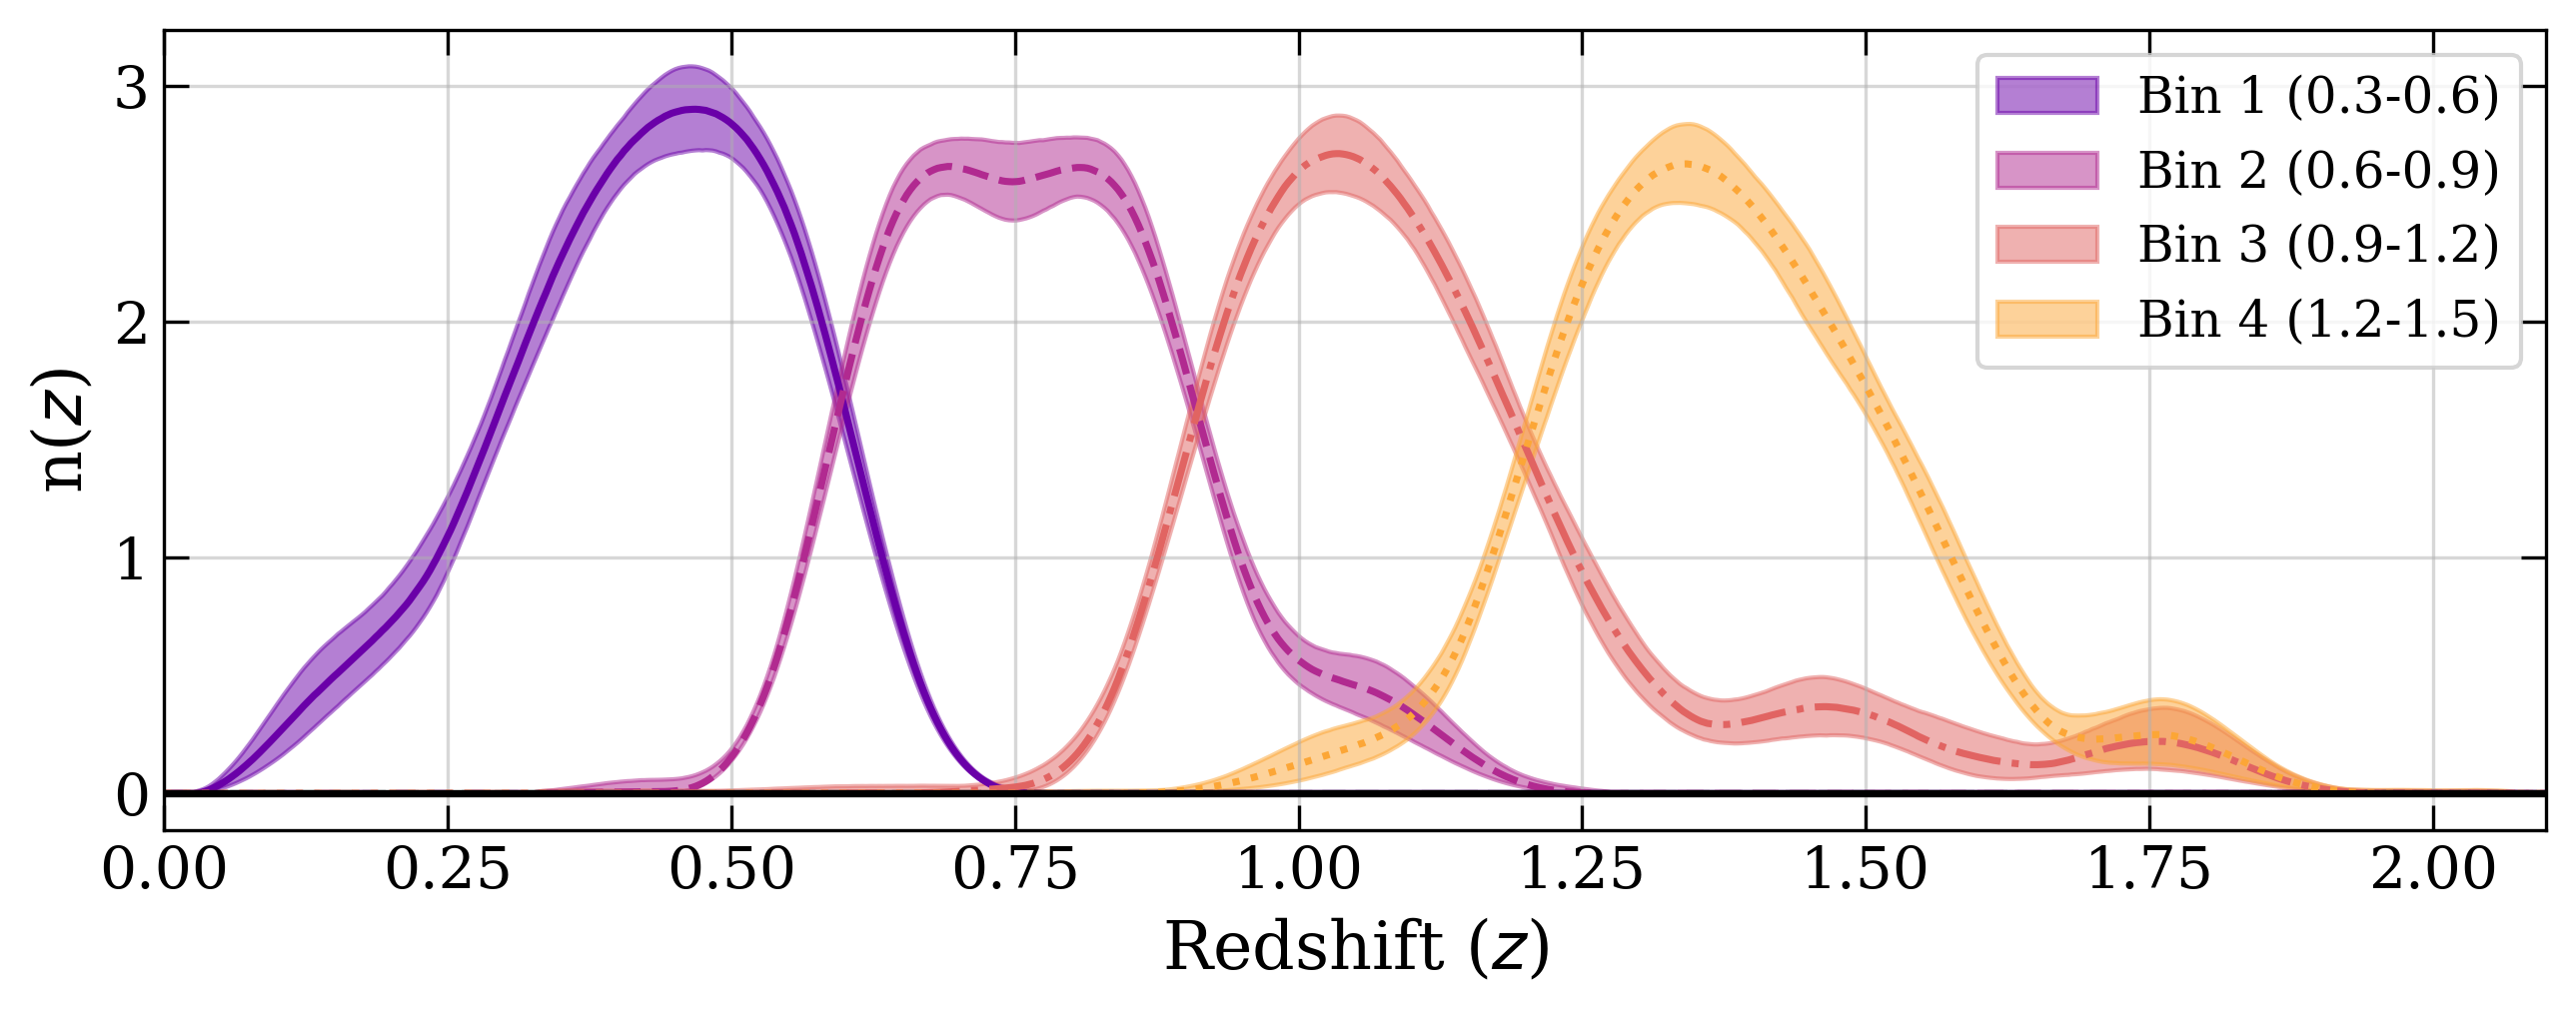
\includegraphics[width=0.95\textwidth]{img/all_tomo_cshear.png}
    \caption{$n(z)$ distributions for each of the 4 tomographic Bins, spanning $z_p\sim0.3$ to $z_p\sim1.5$ where $z_p$ is the best estimate of the \texttt{DNNz} photo-$z$ algorithm \cite{DNNZHSCNishizawa2020} used for tomographic Bin selection, as described in section \ref{sec:data:hsc}. The $n(z)$ for each Bin is displayed with the median posterior sample and the $1\sigma$ widths adapted from \cite{ChoppinDeJanvry2025a}. Here, the $n(z)$ shown includes all corrections to galaxy bias and magnification effects.}
    \label{fig:all_tomo}
\end{figure}

We analyze how the cross-correlation amplitude varies with spectroscopic redshift, characterize and model systematic biases (including galaxy bias from both the spectroscopic and photometric samples and magnification effects) and finally, we reconstruct a fully DESI-calibrated underlying redshift distribution $n(z)$ of the four tomographic bins of the HSC Y3 photometric sample, displayed in figure \ref{fig:all_tomo}. In the clustering redshifts analysis, we include two scale cuts used for two-point correlation functions in the $n(z)$ calibration measurement ($0.3-3$h$^{-1}$Mpc and $1-5$h$^{-1}$Mpc). The smaller scale cut remains the fiducial measurement of this work: however, we make use of both scale cuts for consistency purposes, as presented in section \ref{sec:results}. For more details on the methodology followed, we refer the reader to Choppin De Janvry {\it et al.} (2025a) \cite{ChoppinDeJanvry2025a}. 

%Compliance with DESI internal policies required the use of DESI DR2 to be limited to the calibration of the two highest HSC tomographic bins: $0.9 < z_{\mathrm{p}}\leq1.2$ and $1.2 < z_{\mathrm{p}}\leq1.5$. We use the public DESI DR1 dataset for the remaining tomographic bins: $0.3 < z_{\mathrm{p}}\leq0.6$ and $0.6 < z_{\mathrm{p}}\leq0.9$. 
%For measurements on tomographic bins different from the fiducial HSC \cite{HSCClusteringRau2023, CosmoShearLi2023HSCY3, Dalal2023CosmoShearHSC} ones (e.g. section \ref{sec:modeling:photoz_gal_bias}), DR1 is used for any tomographic bin such that $z_{\mathrm{p}}\lesssim0.9$, and DR2 elsewhere ($z_{\mathrm{p}}>0.9$), where $z_{\mathrm{p}}$ is the center of the tomographic bin. 
%The DESI dataset is further described hereafter, in section \ref{sec:data:desi}. 
%The photometric sample we calibrate is the S19A HSC-SSP PDR3 Shape Catalog (HSC) \cite{HSCShapeCataloguePDR3Li2022}, described in \ref{sec:data:hsc}. Each of the three catalogs is displayed in Figure \ref{fig:footprint}.


%\begin{figure}[h]
%    \centering
%    
\includegraphics[width=0.95\textwidth]{img/sec2/footprint.png}
%    \caption{Sky coverage of DESI DR1 (navy outline), DR2 (in background density map, including all target classes in the number of galaxies $\mathrm{N}_g$) and HSC Year 3 (red outline), with the galactic plane (gray line). The HSC data lands in areas of high overall completeness for DESI, as these areas were targeted in priority. DESI DR2 improves over DR1 with better overall completeness, especially for the ELGs and in the northern \texttt{HECTOMAP} field (roughly $\mathrm{RA}\sim40^\circ$, $\mathrm{DEC}\sim240^\circ$).}
%    \label{fig:footprint}
%\end{figure}

%For both DESI DR1 and DR2, calibrations are performed with the Large Scale Structure (LSS) catalogs of the DESI survey \cite{DESIConstructionLSS2024}. The LSS catalogs provide weighted clustering and random catalogs tailored to the specifics of the DESI survey for each of the target classes %(and sub targets) 
%used. The LSS catalogs take into account imaging systematics, selection and footprint effects, possible redshift failures, tiling overlap, as well as other effects -- the full description of which can be found in the DESI data model\footnote{\href{https://desidatamodel.readthedocs.io/en/latest/DESI_ROOT/survey/catalogs/RELEASE/LSS/SPECPROD/LSScats/VERSION/data_clustering.html}{\textcolor{blue}{https://desidatamodel.readthedocs.io/}}} and in in refs \citep{DESIConstructionLSS2024, DESI.2024.II.SampleDef}. 

%This work uses multiple target classes: the BGS  \cite{DESI.Selection.BGS.Hahn2023}, the LRGs \cite{DESI.Selection.LRG.Zhou2023}, the ELGs \cite{DESI.Selection.ELG.Raichoor2023} and the QSOs \cite{DESI.Selection.QSO.Chaussidon2023} as described above. 
%The target classes redshift ranges used in this study are described in Table \ref{tab:desi_z_bounds}, per data release, and the redshift density distribution for both data releases over the HSC footprint is showcased in Figure \ref{fig:density_z}. 
%DESI uses priority ranking to perform fiber assignment on targets \cite{FiberSystem.Poppett.2024}. 
%For the ELG sample, our analysis uses the LOw-Priority (LOP) sample \cite{DESI.Selection.ELG.Raichoor2023} when calibrating with DR1, which has a selection of higher priority ELGs at $1.1\lesssim z\lesssim1.6$. 
%For DR2, in addition to LOP, we use the Very LOw priority (VLO) sample for ELGs, which focuses on targets in $0.6\lesssim z\lesssim1.1$. Indeed, the addition of VLO to the LSS catalogs is a new feature of DR2 compared to DR1.

%\begin{table}[h]
%\centering
%\caption{Redshift ranges as inclusive bin edges used for each data release per tracer.}
%\begin{tabular}{c|c|c}
%\hline
%\textbf{Tracer} & \textbf{DR1} & \textbf{DR2} \\
%\hline
%BGS & $0-0.5$ & $0-0.6$ \\
%LRG & $0.4-1.1$ & $0.3-1.2$ \\
%ELG (LOP) & $0.8-1.6$ & - \\
%ELG (LOP+VLO) & - & $0.7-1.6$ \\
%QSO & $0.8-2.8$ & $0.7-2.8$ \\
%\end{tabular}
%\label{tab:desi_z_bounds}
%\end{table}

%Note that for DR2, some sources are expected outside of the bounds described in Table \ref{tab:desi_z_bounds} and shown in Figure \ref{fig:density_z}.
%Their lower number densities and negligible overlap with the two highest redshift tomographic bins of HSC motivates our choice for redshift cuts. 
%For example, information from low redshift ELGs ($\lesssim0.7$) is not included.


%\begin{figure}[ht]
%    \centering
%    
\includegraphics[width=0.95\textwidth]{img/sec2/density_z.png}
%    \caption{\textit{Upper panel:} N(z) angular density per redshift from the HSC catalog, using photometric redshifts from the \texttt{DNNz} algorithm \cite{DNNZHSCNishizawa2020}. The effect of the calibration cut on HSC is displayed, removing problematic sources up to $z_{\mathrm{best}}^{\mathtt{DNNz}}\leq0.9$ (dotted histogram), as well as HSC's four tomographic bins (shaded colors, including the calibration cut). \textit{Lower panel:} N(z) angular density per redshift of the DESI Large Scale Structure clustering catalogs \cite{DESIConstructionLSS2024}, showcasing the combined tracers distribution (light blue) in the HSC footprint and individual tracers (BGS, ELG, LRG and QSOs). DR1 is represented in dotted lines and DR2 is represented in full lines. In this figure, ELGs are distinguished between ELG-LOP (DR1 analysis) and ELG-LOP+VLO (DR2 analysis). Since most of the HSC footprint is already included in DR1, adding DR2 does not provide an improvement as big as one could expect (cf.  Figure \ref{fig:footprint}). Per tomographic bins, the effective number density counts are 3.77, 5.07, 4.00 and 2.12 arcmin$^{-2}$ \cite{PSFModellingHSCZhang2023} after applying the calibration cut.}
%    \label{fig:density_z}
%\end{figure}


\section{Method}
\label{sec:method}

%\todo{Present the methodology used to recover the P(k) and extrapolate cosmological constraints}
%\tianqing{I think the methodology should be presented in two sub-sections, one for importance weighting, one for the likelihood analysis. I have taken the liberty to re-organize these text.}
%\jean{I agree. Thank you for this change. Should we cover anything about the theoretical basics, or do we delegate this to citing Li+2023 ?}
%\sgg{Delegate to Li+2023.}

This section presents the methodology followed in this analysis to recover cosmological constraints. We obtain cosmological constraints in two independent approaches: (a) In Section~\ref{sec:method:importance}, we apply importance weighting to the redshift distribution parameters of the fiducial HSC Y3 cosmic shear chains \cite{Li2023_HSCY3_CosmicShear,Dalal2023CosmoShearHSC} based on our new redshift parameter priors; (b) in Section~\ref{sec:method:mcmc}, we re-run likelihood analysis using the fiducial HSC cosmic shear, with our updated redshift distribution and redshift parameter priors. 


\subsection{Importance Weighting}
\label{sec:method:importance}

Our first approach is to apply importance weights to the photometric redshift shifts $\Delta z$ on the original chains \cite{Li2023_HSCY3_CosmicShear}. The importance weights are only applied to the last two tomographic bins, leveraging the broad uniform ($\mathcal{U}(-1,1)$) that were applied to the shift parameters in the original analysis. No resampling is applied to the first two bins, because of their narrow gaussian prior already set by original HSC analysis. Bin 1's new calibration presents a slight shift compared to the original $n(z)$ presented in \cite{HSCClusteringRau2023}, but does not offer significant cosmological information due to being at low redshifts ($0.3\lesssim z\lesssim0.6$), so reweighting for bin 1 is neglected. Bin 2's calibration is fully consistent with the calibration presented by Cosmic Shear Ratios \cite{Rana2025HSCY3CosmicShearRatios} and the original calibration \cite{HSCClusteringRau2023}. The obtained result is also consistent with the sampling result, as shown in section \ref{sec:results}, however, the posterior volume is larger, attributed to larger priors on the first two Bins. The weights $w^{(k)}_i$ derived for Bin $k\in\{3,\,4\}$ are:
\begin{equation}
    w^{(k)}_i=e^{\left(\frac{\mu^{(k)}_i-\mu^{(k)}}{\sigma^{(k)}}\right)}
\end{equation}
where $\mu^{(k)}_i$ is the mean redshift shift of Bin $k$ of posterior draw $i$ from the original chain, $\mu^{(k)}$, $\sigma^{(k)}$ are respectively the mean and standard deviations of the new prior. Since no weighting is originally applied from the uniform prior, we can multiply the existing weights in MCMC chains with $w^{(k)}_i$.

\subsection{Likelihood Analysis}
\label{sec:method:mcmc}

Our second approach towards cosmological parameter inference is to re-run the HSC Y3 fiducial likelihood analysis with our DESI-calibrated redshift distribution $n(z)$ for all four tomographic bins. 

The real-space cosmic shear likelihood analysis follows the setup presented in \cite{Li2023_HSCY3_CosmicShear} as close as possible, which enables us to highlight the effects caused solely by the photometric redshift calibration. Our analysis setup follows the modeling choices in \cite{Li2023_HSCY3_CosmicShear} in terms of the calculation of the Baryonic physics, galaxy intrinsic alignment, shear multiplicative bias, and PSF additive bias. 
For all parameters besides the photo-$z$ parameters, we follow the choices performed in \cite{Li2023_HSCY3_CosmicShear, Dalal2023CosmoShearHSC} and implement a total of 23 free parameters. The cosmological inference is implemented in the public software \texttt{CosmoSIS}\footnote{\href{https://github.com/cosmosis-developers/cosmosis-standard-library}{\textcolor{blue}{github.com/cosmosis-developers/cosmosis-standard-library}}} and the configuration files used in this analysis are made available through the common repository for this work and the companion $n(z)$ calibration analysis \citep{ChoppinDeJanvry2025a}: \href{https://github.com/JeanCHDJdev/desi-y3-hsc}{\textcolor{blue}{github.com/jeanchdjdev/desi-y3-hsc}}. The priors for all of the 23 parameters are described in table \ref{tab:post}. The fixed parameters are given in table \ref{tab:fixed} in appendix \ref{sec:appendix}.
For the matter power spectrum, we use the CAMB\footnote{\href{https://camb.info/}{\textcolor{blue} {camb.info}}} \cite{LewisCAMB2011} linear power spectrum emulator, in a divergent approach from using the BACCO suite of emulators  \cite{Arico2022BACCOEmulator} \footnote{\href{https://baccoemu.readthedocs.io/en/latest/}{\textcolor{blue}{baccoemu.readthedocs.io}}} used in \cite{Li2023_HSCY3_CosmicShear}. It is shown that there is no significant different in cosmology results between CAMB and BACCO emulator for HSC Y3 \cite{Li2023_HSCY3_CosmicShear}.


The two-point correlation functions (TPCF) of galaxy shear are denoted $\xi_\pm$ \cite{Li2023_HSCY3_CosmicShear} and are measured on the shear catalog introduced in section \ref{sec:data:hsc}.
We also follow the same formalism when it comes to likelihood calculation, compared to \cite{Li2023_HSCY3_CosmicShear}.
The scale cut applied in this analysis is the same as  \cite{Li2023_HSCY3_CosmicShear}: $7.1 < \theta < 56.6$ [arcmin] for $\xi_+(\theta)$, and $31.2 < \theta < 248$ [arcmin] for $\xi_+(\theta)$. We adopted the same covariance matrix calculated by 1404 mock HSC Y3 catalogs. We also apply the same Hartlap factor \cite{Hartlap2008} to the likelihood calculation to account for covariance matrix underestimation due to limited mock catalogs. In the HSC Y3 fiducial pipeline, the $S_8$ parameter is not sampled and is instead a computed property from the other sampled parameters. 

%\subsection{Sampling}
The sampler we used for the likelihood analysis is \texttt{pocoMC}\footnote{\href{https://pocomc.readthedocs.io/en/latest/}{\textcolor{blue}{pocomc.readthedocs.io}}} \cite{karamanis2022pocoMC1, karamanis2022pocoMC2}. \texttt{pocoMC} utilizes the Preconditioned Monte Carlo (PMC) algorithm which offers significant speed-ups over more traditional approaches such as Markov Chain Monte Carlo (MCMC). We verify \texttt{pocoMC} accurately recovers the fiducial HSC chains in \texttt{CosmoSIS}. 2D posteriors for parameters are obtained with the \texttt{getDist}\footnote{\href{https://getdist.readthedocs.io/en/latest/}{\textcolor{blue}{getdist.readthedocs.io}}} \cite{getDistLewis2025} package. Comparatively to \cite{Li2023_HSCY3_CosmicShear}, this work does not use the \texttt{ChainConsumer}\footnote{\href{https://samreay.github.io/ChainConsumer/}{\textcolor{blue}{samreay.github.io/ChainConsumer/}}} \cite{ChainConsumer_Hinton2016} package to treat the chains, due to potential biases incorporated by the boundary effects and smoothing of MC samples at the border with Kernel Density Estimation (KDE) mentioned in Appendix A of \cite{Li2023_HSCY3_CosmicShear}. However, constraints are also computed with \texttt{ChainConsumer} and consistency with \texttt{getDist} is confirmed for parameters $S_8$ and $\Omega_m$.

In this work, the posterior of cosmological parameter constraints is presented in the form of:
\begin{equation}\label{eq:presentation}
    \text{1D mode} ^ {+34\%} _ {-34\%}\;\text{(MAP)}
\end{equation}
where the 1D mode is the is 1D mode of the marginalized 1D posterior distribution, the MAP is the Maximum A Posteriori point of the chain, and the error interval is the asymmetric $34\%$ confidence interval obtained with the $68\%$ interval from the cumulative density function. The values themselves are presented as obtained by \texttt{getDist} using \texttt{MCSamples.get1DDensity} and the weights are obtained through the sampling from \texttt{pocoMC} or included in the fiducial HSC Y3 chains.


\section{Results}
\label{sec:results}

In this section, we present the fiducial constraints we obtain from the weak lensing cosmological inference in real space and compare them to other experiments and surveys. Measurements from this analysis are compared to other, comparable measurements in order to obtain precise joint constraints of the growth of structure. 

\begin{figure}[ht]
    \centering
    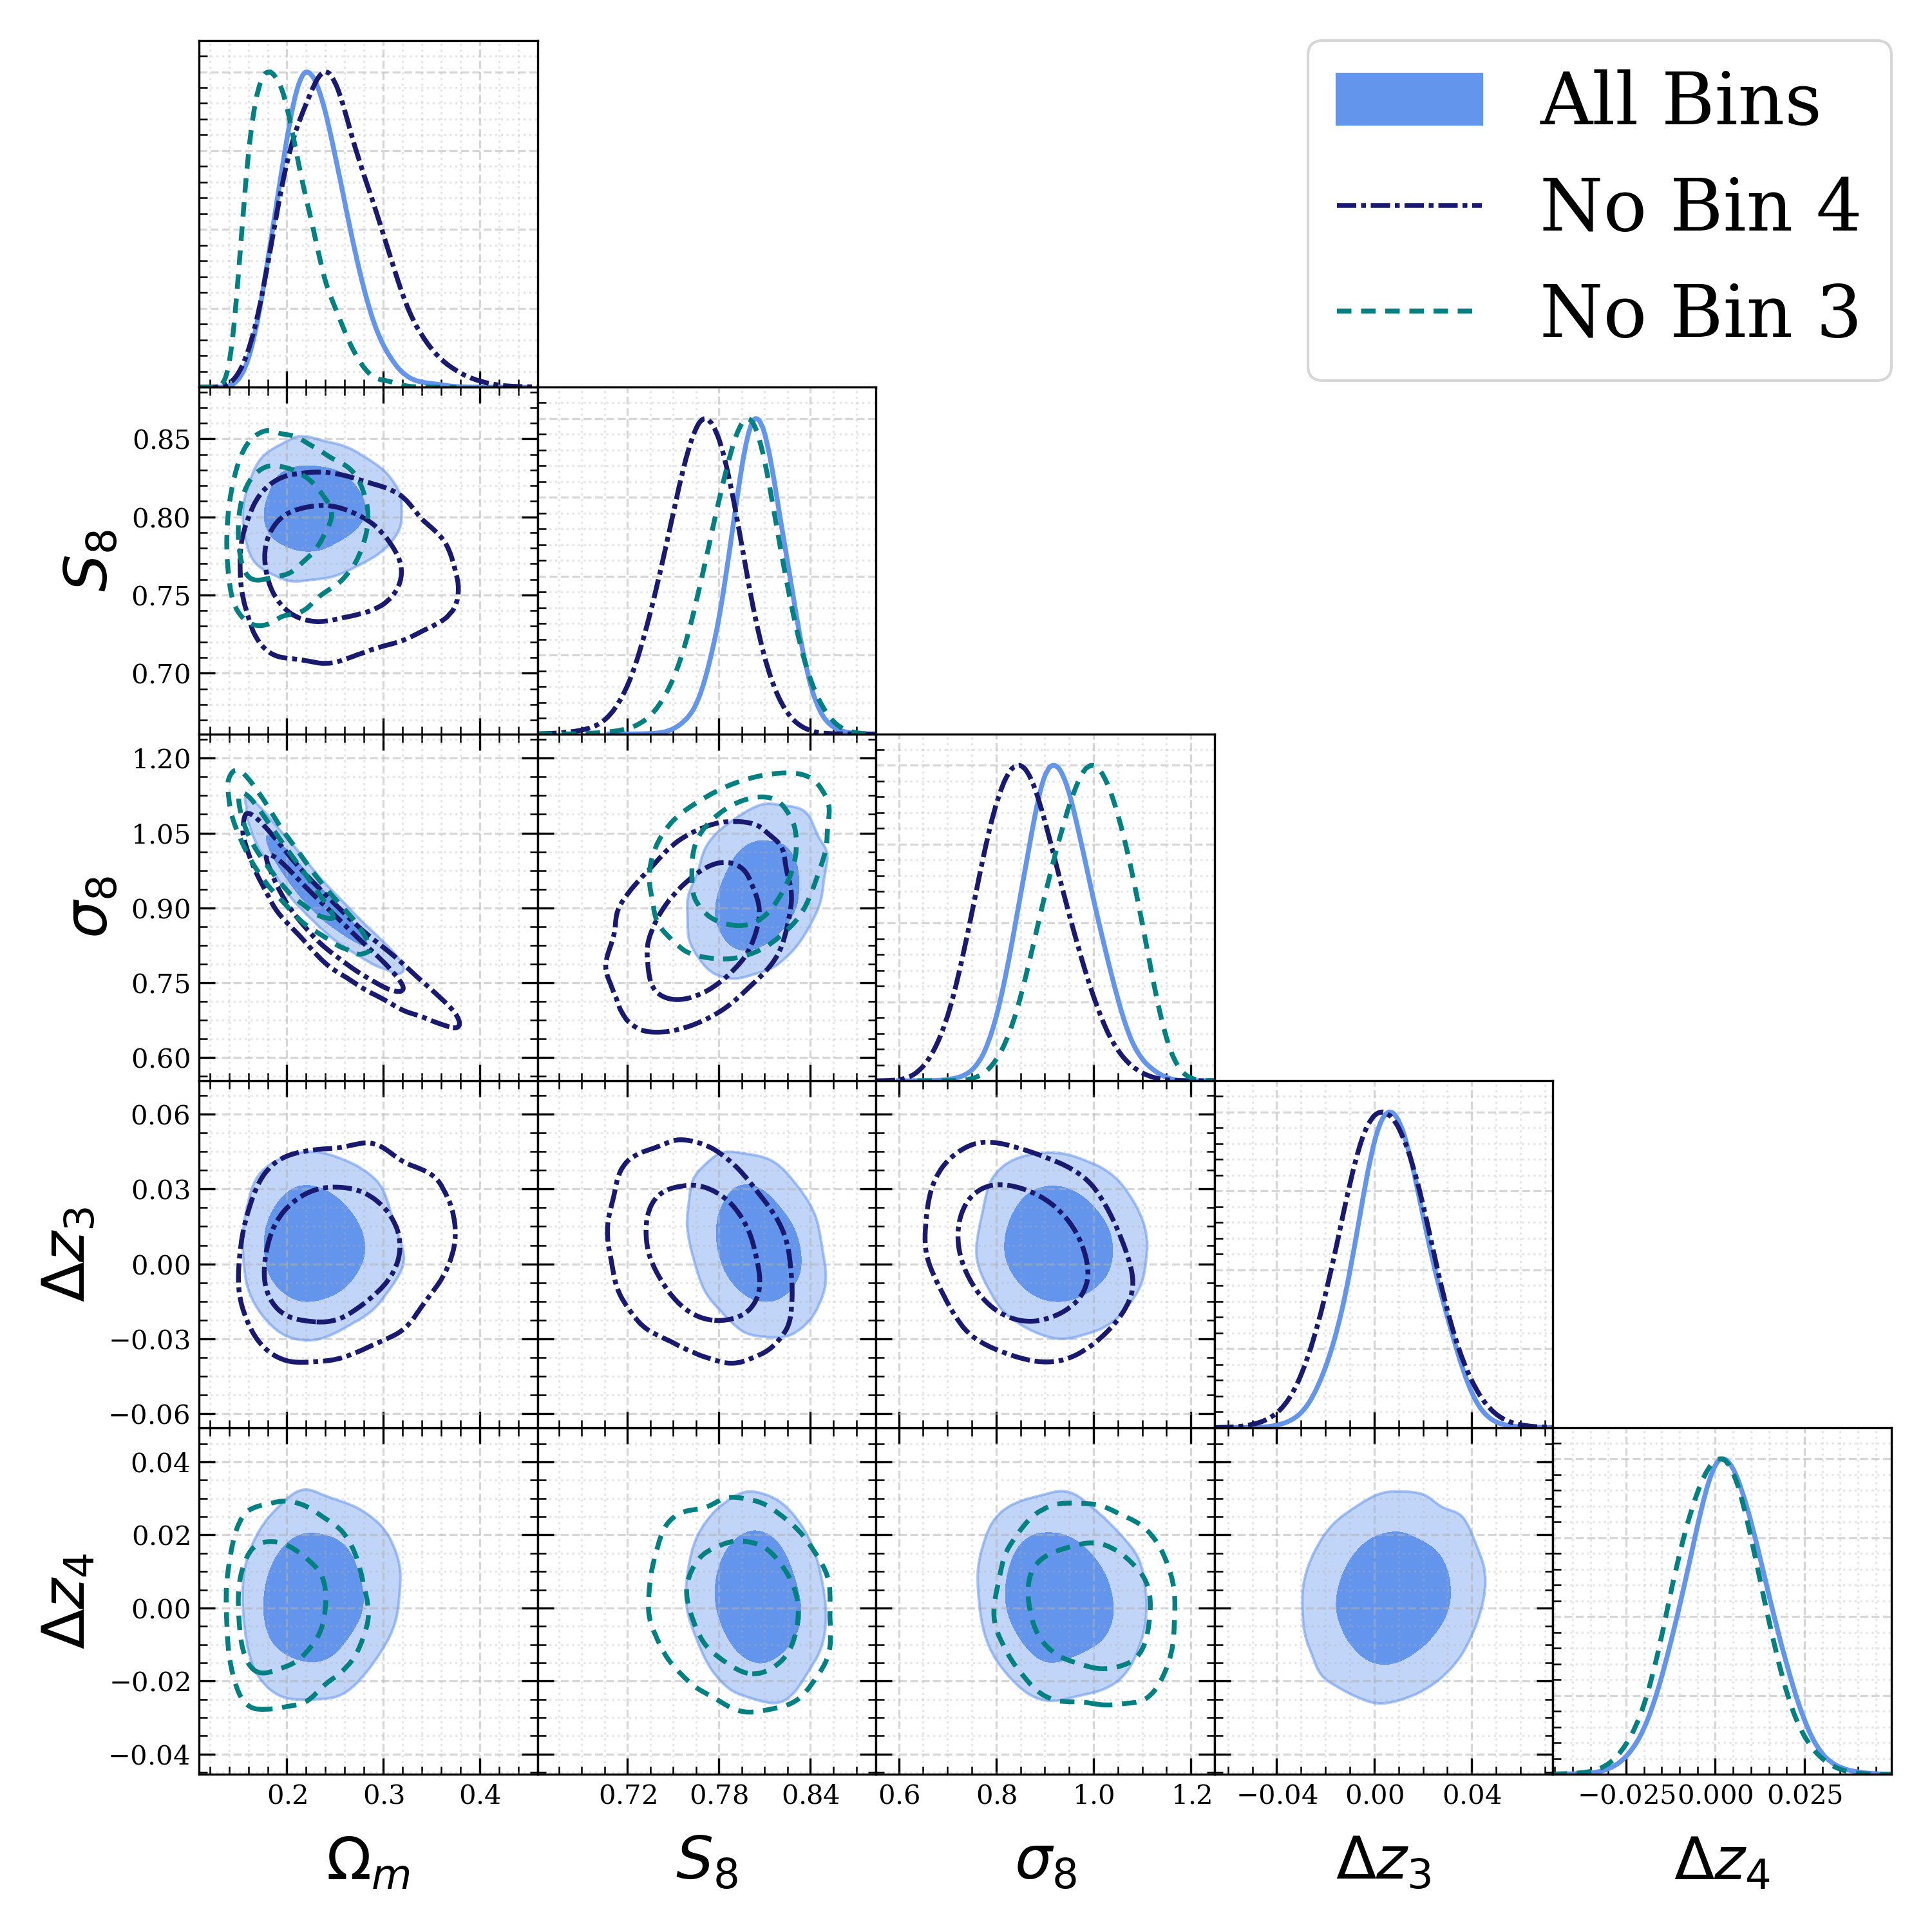
\includegraphics[width=0.9\textwidth]{img/corner_excluded_bins.png}
    \caption{To assess the robustness of the measurement, we exclude Bin 3 and Bin 4 respectively from the chain inference. The measurements are shown to be consistent between the two and consistent with the "All Bins" measurement.}
    \label{fig:corner_excluded_bins}
\end{figure}

Furthermore, we investigate the robustness of this analysis by comparing the results to importance sampling of the fiducial chains, as well as using different configuration for the tomographic $n(z)$ distributions. We note that following the setup proposed in \texttt{CosmoSIS}, the convention used for $\Delta z$ parameter shifts is opposed to the one presented in the clustering redshift analyses \cite{HSCClusteringRau2023, ChoppinDeJanvry2025a} and in the cosmological inference works such as \cite{Li2023_HSCY3_CosmicShear, Dalal2023CosmoShearHSC, Zhang2025aTomographic2x2pt, Zhang2025bTomographic3x2pt}. Here, a positive shift implies that the real $n(z)$ distribution is at higher redshifts than the original, calibrated one proposed in the redshift calibration analyses: the original convention implied the same for negative shifts.

\begin{figure}[ht]
    \centering
    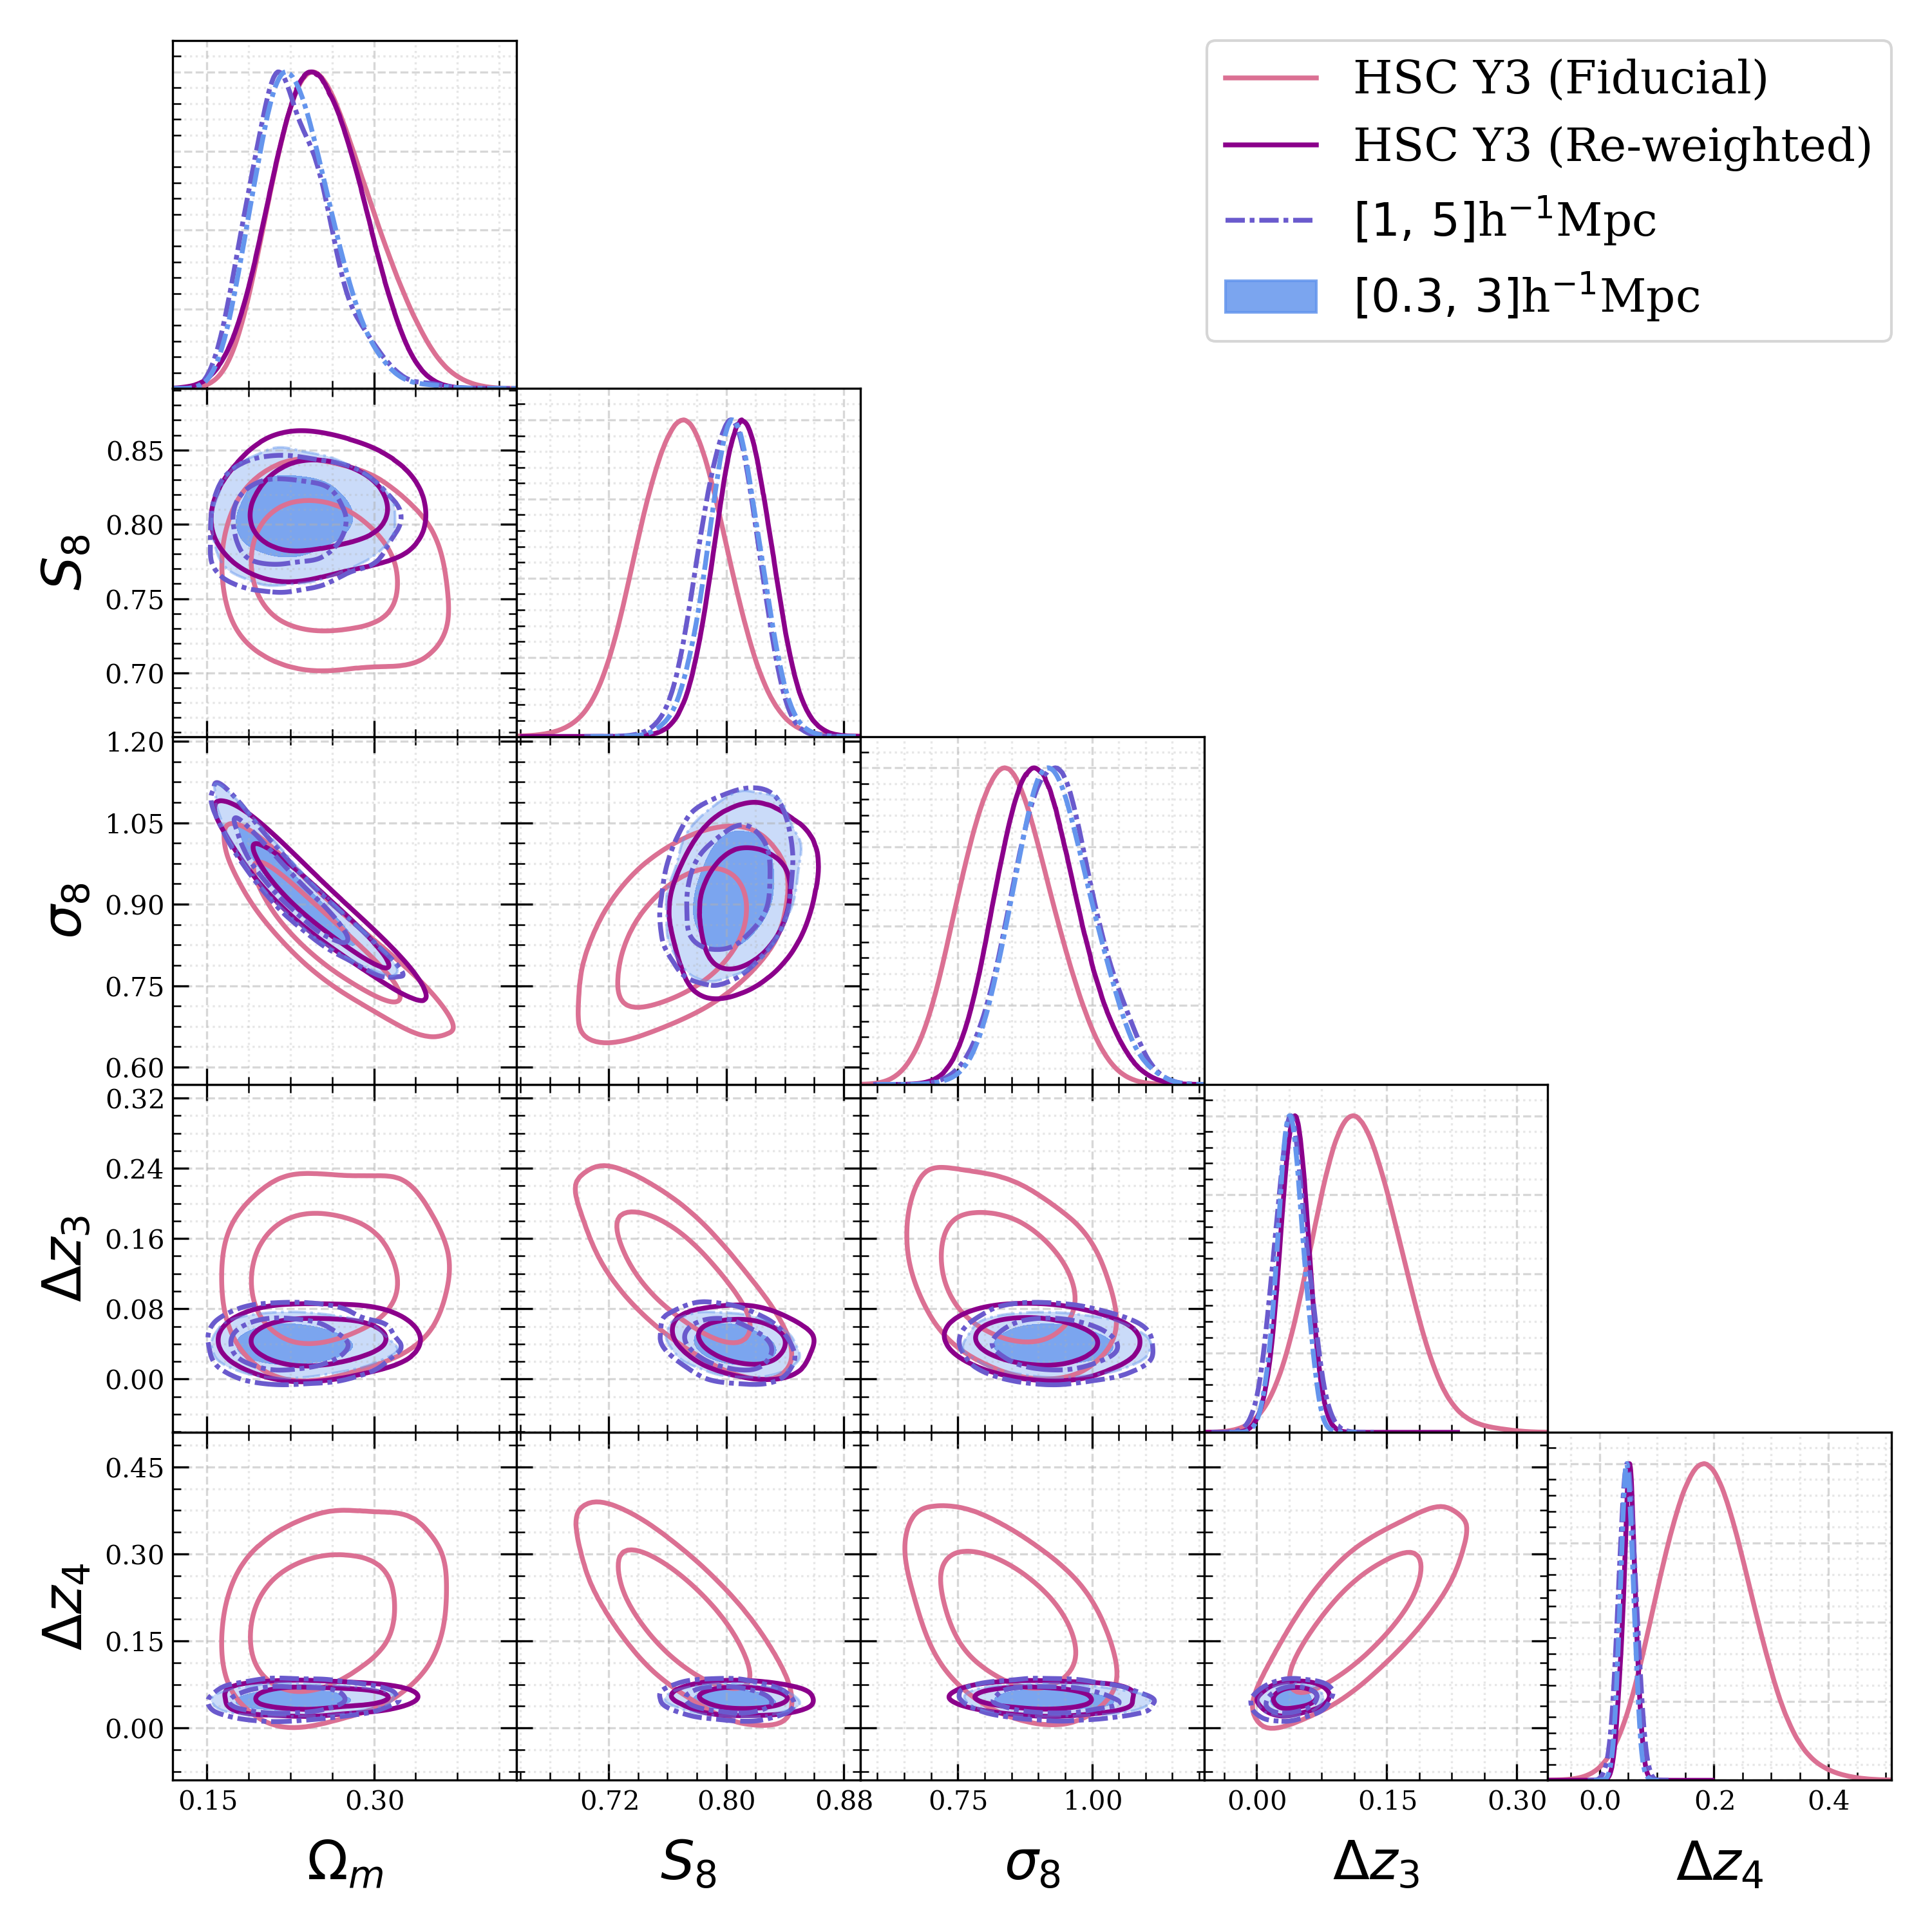
\includegraphics[width=0.95\textwidth]{img/compare_resampling_sc.png}
    \caption{Comparing the sampled results (section \ref{sec:method:mcmc}) from the two $n(z)$ set of distributions at different scale cuts with the importance re-weighting (section \ref{sec:method:importance}) approach in real space and to  the HSC Y3 fiducial result. The shift posteriors are artificially shifted by the expectation of the inferred shift in \cite{ChoppinDeJanvry2025a}, as they are by default centered around 0 for the sampling approach, since new $n(z)$ distributions are used.}
    \label{fig:corner_resampling_sc}
\end{figure}

Figure \ref{fig:corner_resampling_sc} compares the joint 2D posteriors for the fiducial result, the $1-5$h$^{-1}$Mpc scale cut $n(z)$ result to the importance sampling in real space and the fiducial HSC Y3 result. The underlying $\Delta z_{\{3,\,4\}}$ shifts lie at 1-2 sigma away from the reported posterior from the HSC Y3. While the shifts are significant in value, they are not statistically inconsistent with the self-calibration 
method deployed in HSC Y3. 

In Figure \ref{fig:corner_excluded_bins}, consistency tests are performed by running cosmological inference while removing information provided by either Bin 3 or Bin 4, and compare to the full run. The resulting corner plot displays consistent measurements between all bins. A preference towards lower $\Omega_m$ and higher $\sigma_8$ values is noticed when excluding Bin 3, akin to behavior presented in Figure 17 of the two-point correlation analysis \cite{Li2023_HSCY3_CosmicShear}, but the $\sigma$-shifts presented in Figure \ref{fig:param_sigma_shifts} alleviate concerns of inconsistencies. The lower error bound of the "No Bin 3" chain is underestimated due to the MCMC chain piling up near the boundaries of the prior ($\pi(\Omega_m)\sim\mathcal{U}(0.1, 0.7)$). Furthermore, the obtained value when excluding Bin 3 presents a fairly low value of $\Omega_m$, showing the same trend as what was obtained in the same scenario in the real space analysis \cite{Li2023_HSCY3_CosmicShear}. In this work, akin to \cite{Li2023_HSCY3_CosmicShear, Dalal2023CosmoShearHSC}, the constraint on the $S_8$ parameter is emphasized, due to the strong degeneracies between parameters $\Omega_m$ and $\sigma_8$.

\begin{figure}[ht]
    \centering
    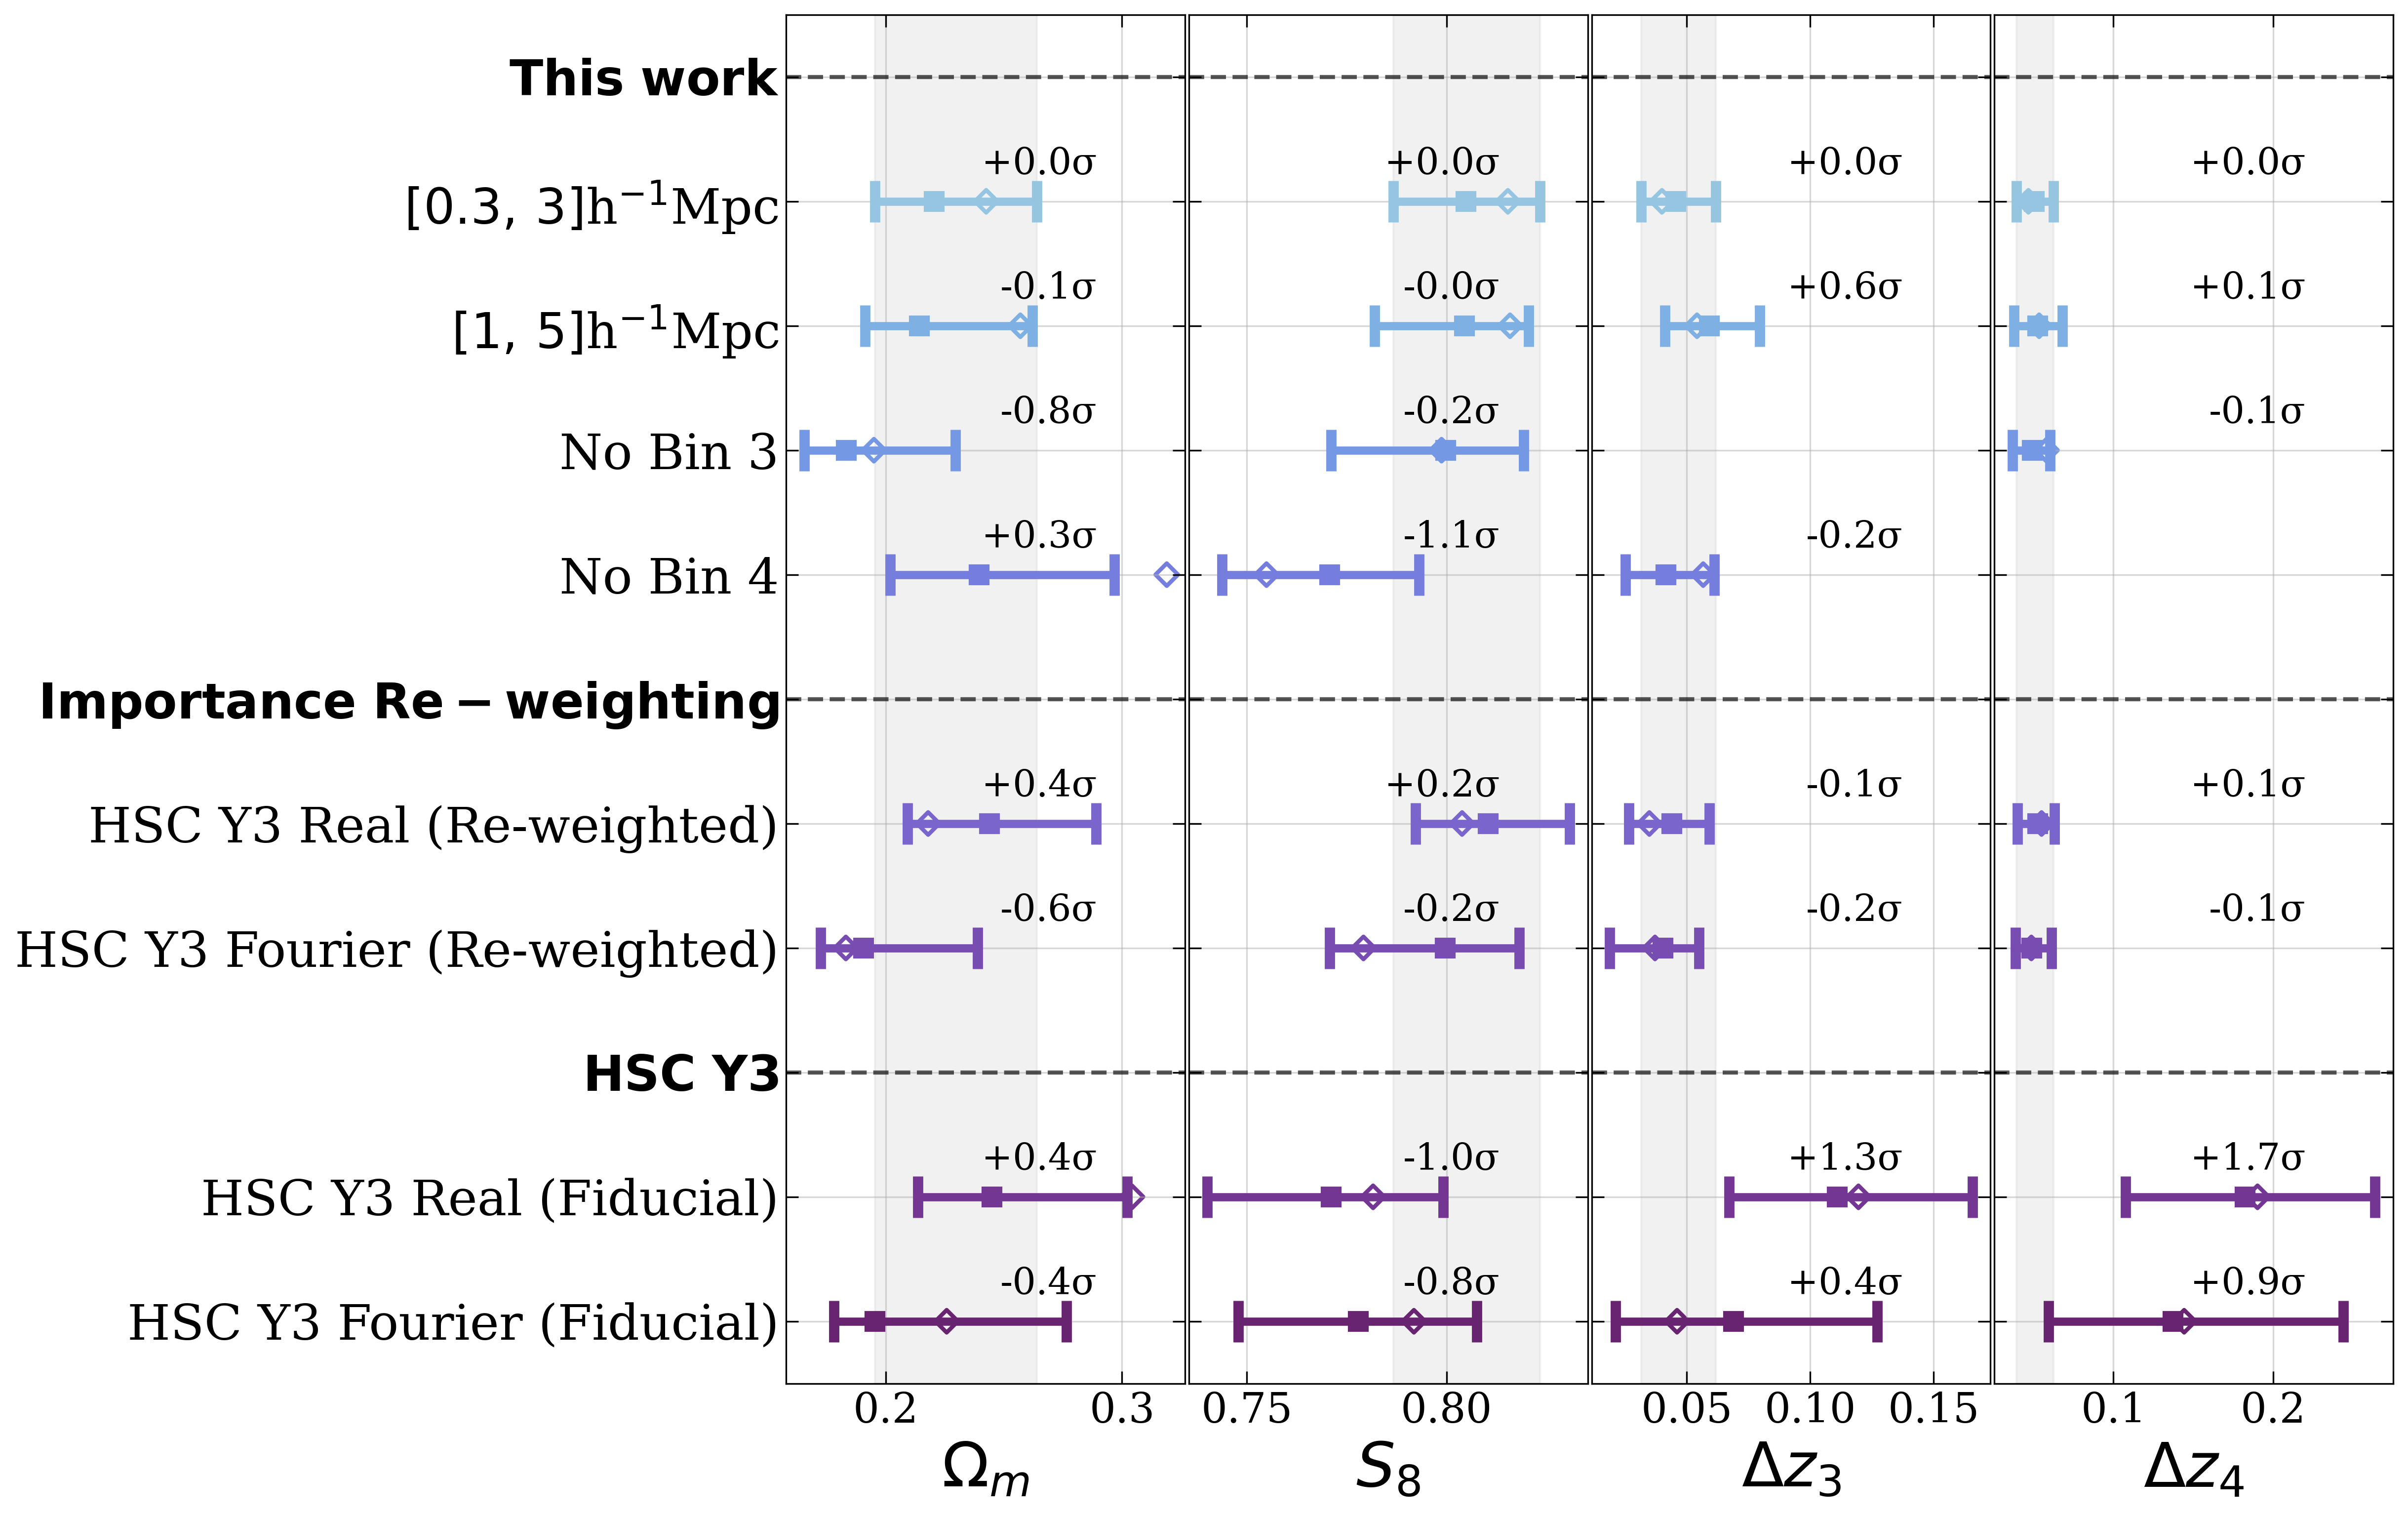
\includegraphics[width=0.95\textwidth]{img/tensions.png}
    \caption{$\Omega_m$, $S_8$, $\Delta z_3$, $\Delta z_4$ parameters compared under different measurements. This includes the sampling approach, where the $n(z)$ distributions at two different scale cuts are included, as well as the measurements obtained when excluding either Bin 3 or Bin 4. These are then compared to the importance re-weighting and fiducial results of the Real and Fourier HSC Y3 analyses \cite{Li2023_HSCY3_CosmicShear, Dalal2023CosmoShearHSC}. The square marker displays the 1D posterior mode obtained with \texttt{getDist}. The diamond marker is the Maximum A Posteriori (MAP) value. The background gray area represents the projected fiducial measurement obtained with the $0.3-3$h$^{-1}$Mpc scale cut for the $n(z)$. The $n(z)$ distributions are not the same for HSC Y3 samples (derived from \cite{HSCClusteringRau2023}) and this work (from \cite{ChoppinDeJanvry2025a}) : the posteriors of this work have been artificially shifted to match the mean of the shifts found in \cite{ChoppinDeJanvry2025a}.}
    \label{fig:param_sigma_shifts}
\end{figure}
%and the $\sigma$ deviations are computed for comparison purposes, assuming gaussian error bars with the error used being the one in the direction of the compared measurement and the distance computed over the reported modes

{\renewcommand{\arraystretch}{1.2}
\begin{table}[ht]
\centering
\caption{\label{tab:post}
Fiducial parameters and priors for this cosmological analysis. 
$\mathcal{U}(a,b)$ represents a flat (uniform) prior over bounds $[a,b]$, while $\mathcal{N}(\mu, \sigma)$ represents a Gaussian prior of mean $\mu$ and standard deviation $\sigma$. $S_8$ and $\sigma_8$ are computed quantities. The values are presented according to equation \ref{eq:presentation}. 
}
\begin{tabular}{l | l | l | l }
\hline
\textbf{Parameter} & \textbf{Prior} & $\mathbf{[0.3,\,3]}$h$\mathbf{^{-1}}$\textbf{Mpc} & $\mathbf{[1,\,5]}$h$\mathbf{^{-1}}$\textbf{Mpc} \\ 
\hline
\hline
\textbf{Cosmological Parameters} &  & & \\
$A_s\,(\times 10^9)$ & $\mathcal{U}(0.5, 10)$ & $3.721_{-0.654}^{+2.221} ({2.765})$ & $3.730_{-0.687}^{+2.410} ({2.922})$ \\ 
$\Omega_m$ & $\mathcal{U}(0.1, 0.7)$ & $0.221_{-0.025}^{+0.043} ({0.243})$ & $0.214_{-0.023}^{+0.048} ({0.257})$ \\ 
$\sigma_8$ & -- & $0.922_{-0.066}^{+0.079} ({0.907})$ & $0.936_{-0.082}^{+0.069} ({0.882})$ \\ 
$S_8$ & -- & $0.805_{-0.018}^{+0.019} ({0.815})$ & $0.804_{-0.022}^{+0.016} ({0.816})$ \\
$n_s$ & $\mathcal{U}(0.87, 1.07)$ & $0.900_{-0.005}^{+0.112} ({0.885})$ & $0.881_{--0.011}^{+0.130} ({0.898})$ \\ 
$h_0$ & $\mathcal{U}(0.62, 0.80)$ & $0.662_{-0.015}^{+0.093} ({0.746})$ & $0.701_{-0.053}^{+0.057} ({0.724})$ \\ 
$\omega_b \equiv \Omega_b h^2$  & $\mathcal{U}(0.02, 0.025)$ & $0.024_{-0.004}^{+-0.000} ({0.020})$ & $0.020_{--0.001}^{+0.004} ({0.024})$ \\ 
\hline
\textbf{Baryonic Feedback} & & & \\
$A_{\rm b}$ & $\mathcal{U}(2, 3.13)$ & $2.075_{-0.024}^{+0.695} ({2.083})$ & $2.041_{-0.054}^{+0.707} ({2.137})$ \\ 
\hline
\textbf{Intrinsic Alignment} & & & \\
$A_1$ & $\mathcal{U}(-6, 6)$ & $0.441_{-0.424}^{+0.272} ({0.648})$ & $0.432_{-0.405}^{+0.341} ({0.503})$ \\ 
$\eta_1$ & $\mathcal{U}(-6, 6)$ & $-2.478_{-1.890}^{+4.117} ({-3.549})$ & $-1.943_{-2.040}^{+3.942} ({-4.323})$ \\ 
$A_2$ & $\mathcal{U}(-6, 6)$ & $-0.058_{-0.652}^{+0.900} ({-0.603})$ & $-0.057_{-0.678}^{+0.925} ({-0.469})$ \\ 
$\eta_2$ & $\mathcal{U}(-6, 6)$ & $-1.524_{-2.330}^{+4.114} ({-3.915})$ & $-1.552_{-2.248}^{+4.352} ({-4.782})$ \\ 
$b_{\rm TA}$ & $\mathcal{U}(0, 2)$ & $0.062_{--0.117}^{+1.371} ({0.061})$ & $0.067_{--0.119}^{+1.392} ({0.163})$ \\ 
\hline
\textbf{Redshift shifts} & & & \\
$\Delta z_1$ & $\mathcal{N}(0, 0.008)$ & $-0.002_{-0.008}^{+0.008} ({-0.002})$ & $-0.003_{-0.013}^{+0.012} ({-0.004})$ \\ 
$\Delta z_1$ & $\mathcal{N}(0, 0.009)$ & $-0.002_{-0.009}^{+0.007} ({-0.009})$ & $-0.010_{-0.012}^{+0.011} ({-0.027})$ \\ 
$\Delta z_3$ & $\mathcal{N}(0, 0.020)$ & $0.007_{-0.014}^{+0.016} ({0.001})$ & $0.020_{-0.018}^{+0.020} ({0.015})$ \\ 
$\Delta z_4$ & $\mathcal{N}(0, 0.012)$ & $0.002_{-0.011}^{+0.012} ({-0.001})$ & $0.005_{-0.015}^{+0.015} ({0.005})$ \\ 
\hline
\textbf{Shear calibration} & & & \\
$\Delta m_1$ & $\mathcal{N}(0, 0.01)$ & $0.000_{-0.011}^{+0.009} ({-0.009})$ & $0.001_{-0.011}^{+0.009} ({-0.003})$ \\ 
$\Delta m_2$ & $\mathcal{N}(0, 0.01)$ & $-0.003_{-0.010}^{+0.009} ({0.001})$ & $-0.005_{-0.010}^{+0.010} ({-0.003})$ \\ 
$\Delta m_3$ & $\mathcal{N}(0, 0.01)$ & $0.000_{-0.009}^{+0.010} ({0.001})$ & $0.001_{-0.009}^{+0.010} ({-0.001})$ \\ 
$\Delta m_4$ & $\mathcal{N}(0, 0.01)$ & $0.005_{-0.009}^{+0.010} ({0.010})$ & $0.007_{-0.011}^{+0.007} ({0.005})$ \\
\hline
\textbf{PSF systematics} & & & \\
$\tilde{\alpha}_2$ & $\mathcal{N}(0, 1)$ & $0.075_{-0.988}^{+0.941} ({0.159})$ & $-0.094_{-0.819}^{+1.123} ({-0.109})$ \\
$\tilde{\beta}_2$ & $\mathcal{N}(0, 1)$ & $0.033_{-0.886}^{+1.016} ({0.160})$ & $0.102_{-1.001}^{+0.927} ({-0.120})$ \\ 
$\tilde{\alpha}_4$ & $\mathcal{N}(0, 1)$ & $-0.347_{-0.850}^{+0.993} ({-1.281})$ & $-0.271_{-0.934}^{+0.920} ({-0.461})$ \\ 
$\tilde{\beta}_4$ & $\mathcal{N}(0, 1)$ & $-0.005_{-1.066}^{+0.911} ({0.271})$ & $-0.091_{-0.971}^{+1.033} ({-0.014})$ \\  
\hline
\end{tabular}
\end{table}}

Figure \ref{fig:param_sigma_shifts} compares the relative shifts to the fiducial measurement of this work under different scenarios. We perform consistency tests with Bin 3 or Bin 4 excluded and using the distributions inferred with the larger scale cut ($1-5$h$^{1}$Mpc) obtained in \cite{ChoppinDeJanvry2025a}. The importance re-weighting results obtained with the method described in section \ref{sec:method:importance} are shown next. The measured shift in the $\Delta z$ bins in the context of the importance re-weighting, the $1-5$h$^{1}$Mpc distributions or in the context of the HSC Y3 fiducial $n(z)$ derived in \cite{HSCClusteringRau2023} cannot be strictly compared to the $n(z)$ shifts found in this work, since the $n(z)$ distributions themselves differ. Lastly, the importance re-weighting of the HSC Y3 chains means constraining the originally broad uniform $\mathcal{U}(-1, 1)$ prior over $\Delta z_3$, $\Delta z_4$ to a stricter gaussian prior. We note that reweighting leads to a fairly low number of effective sample size with respect to the original chain, leading to noisy 2D posteriors. 

\begin{figure}[ht!]
    \centering
    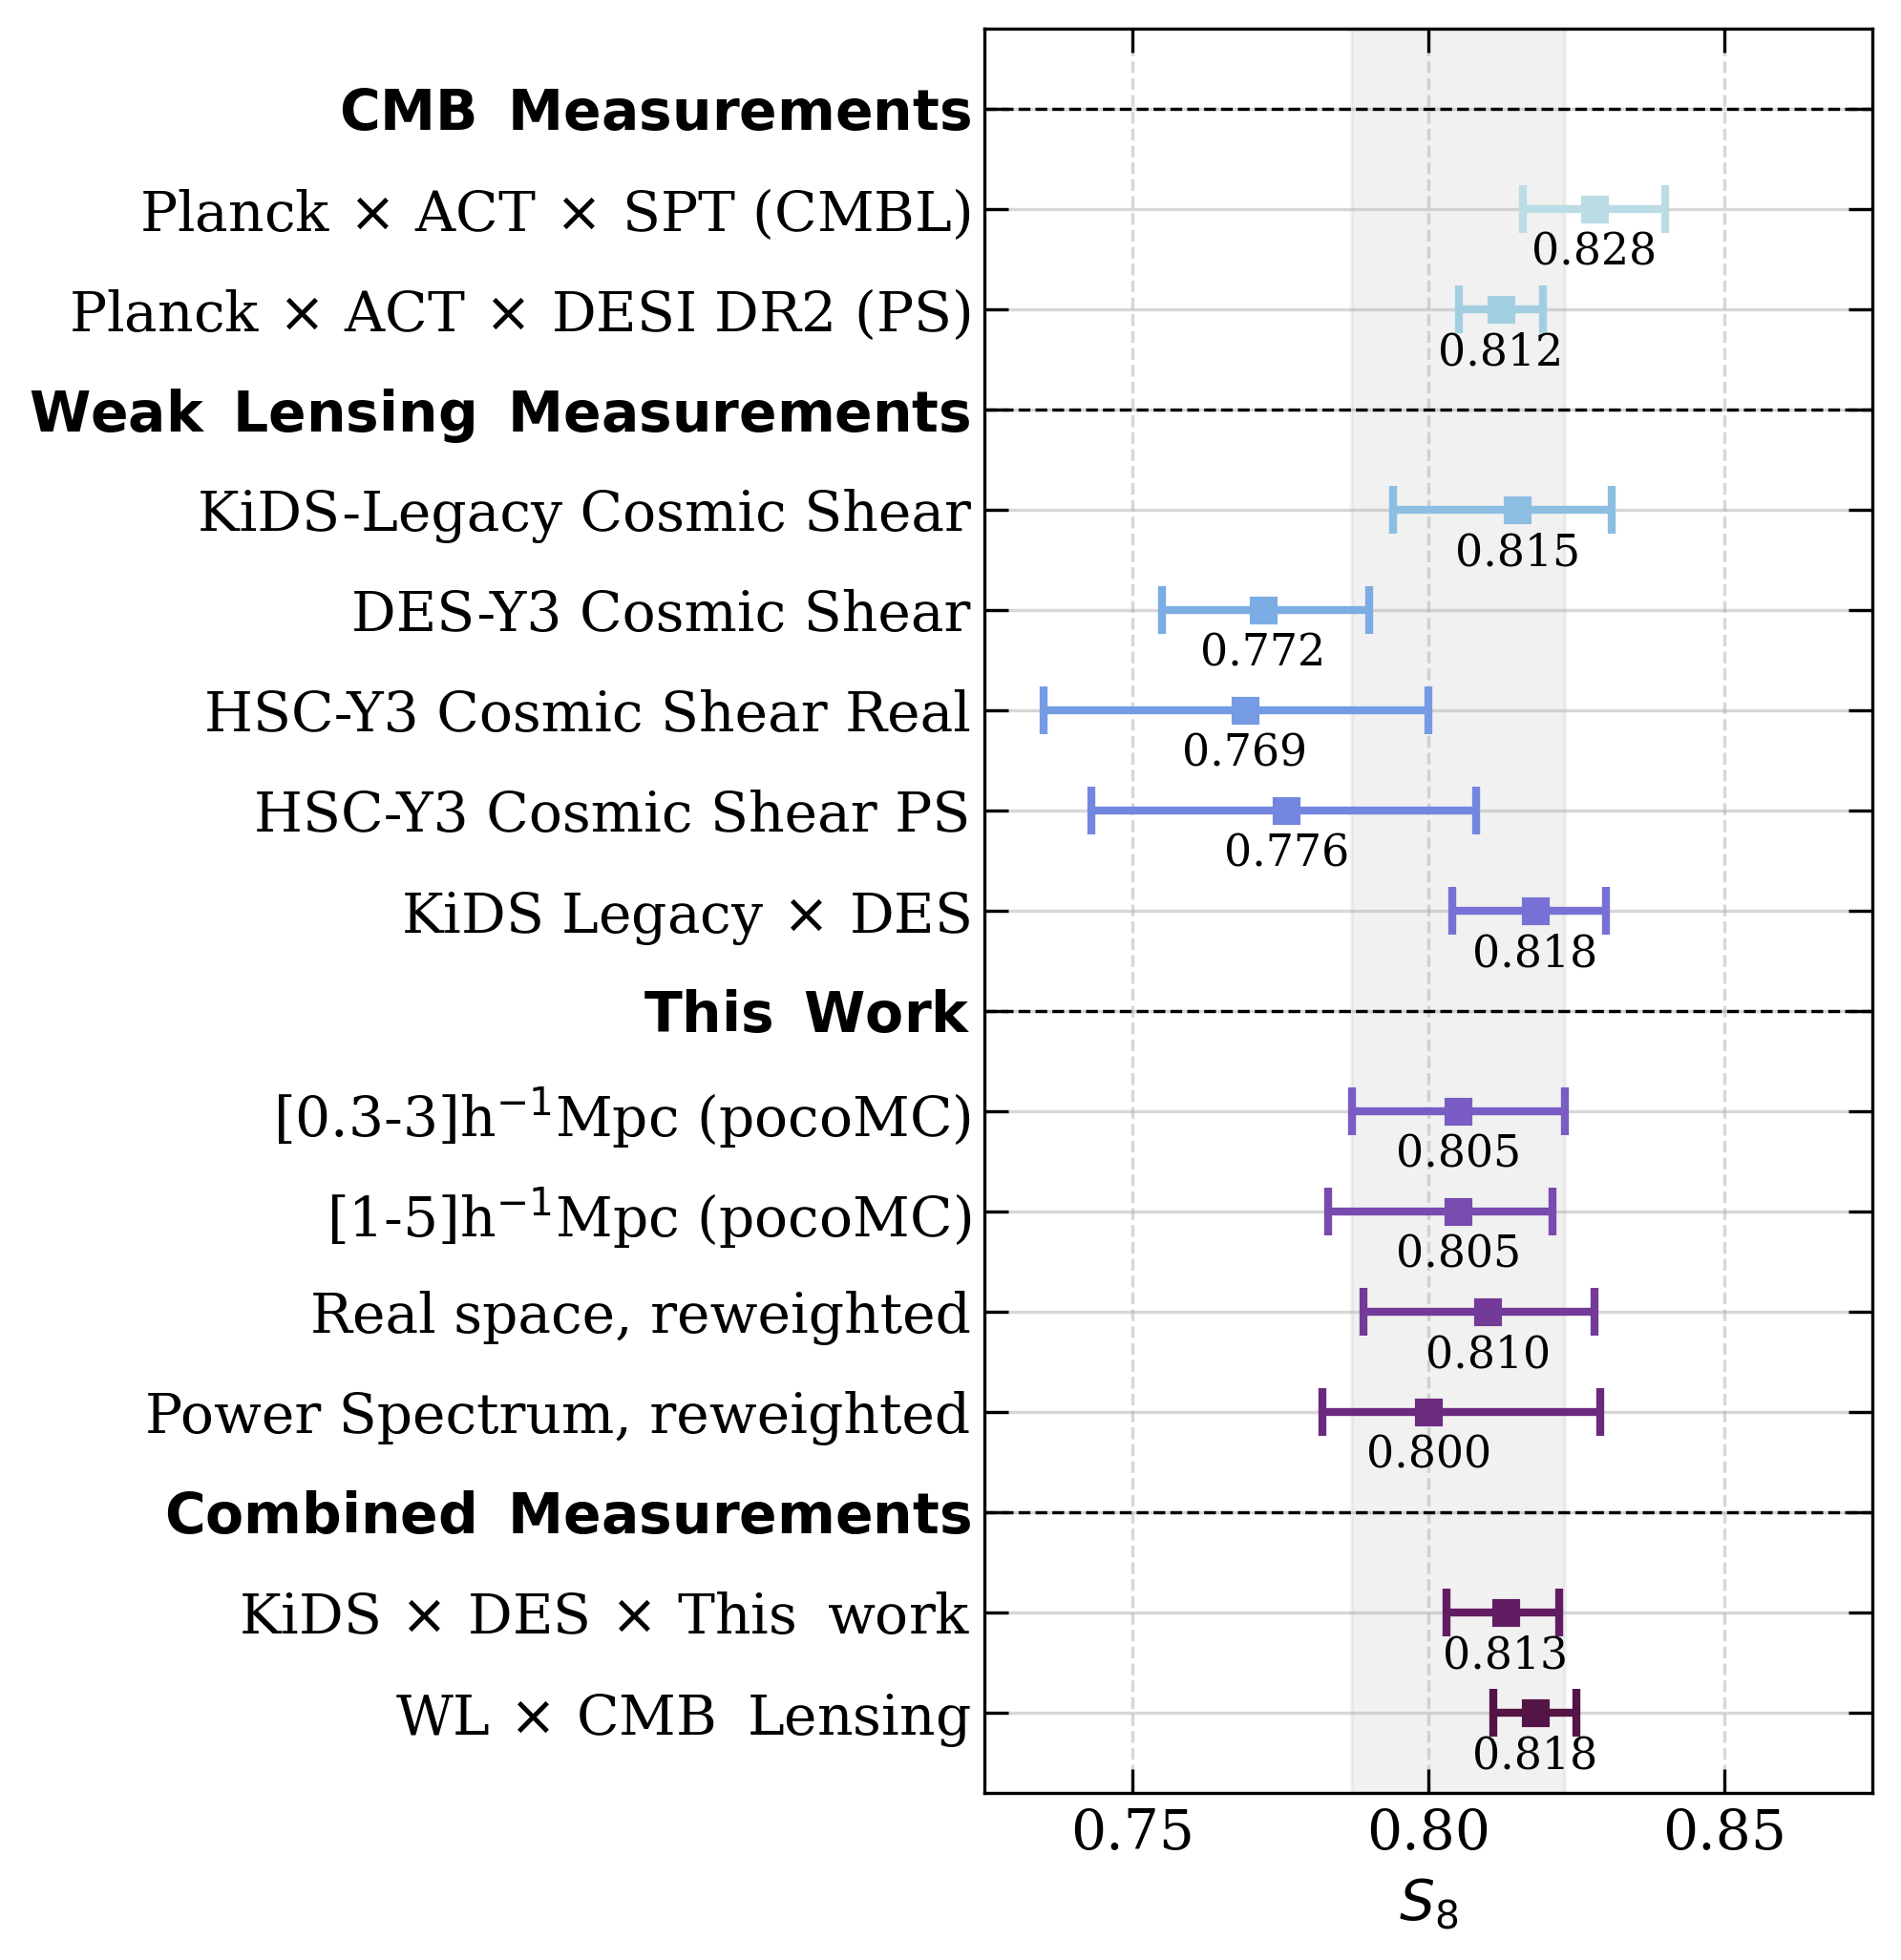
\includegraphics[width=0.95\textwidth]{img/comparison_s8.png}
    \caption{Measurements from different surveys measuring the growth of structure, from \textit{CMB Measurements} and \textit{Weak Lensing Measurements}. The results are further compared to the results obtained in this work, as well as combined with the $S_8$ constraints obtained. The  source of every cited measurement is discussed in text.}
    \label{fig:comparison_S8}
\end{figure}

The priors for all sampled parameters in the case of the fiducial $n(z)$ is reported in table \ref{tab:post}, alongside the posterior sampled values obtained for the other scale cuts. We note that the redshift $\Delta z_i$ priors depend on the chosen scale cut, as mentioned in appendix \ref{sec:appendix}.
Figure \ref{fig:comparison_S8} compares other recent $S_8$ constraints with respect to the constraints obtained in this work.  The most recent non-lensing CMB result is Planck $\times$ ACT $\times$ DESI DR2 constraints obtained from the power spectra measurements of ACT DR6 presented in \cite{Louis2025_ACTDR6_PS_S8}. The 
most recent CMB lensing result is Planck $\times$ ACT $\times$ SPT (CMBL): the CMB lensing constraints obtained from combining Planck, ACT and SPT maps in work \cite{Qu2025_ACTSPTPLANCK_CMBL_S8}.
We also show measurements obtained with weak lensing from KiDS-Legacy \cite{Wright2025_KiDSLegacy}, DES \cite{Amon2022CosmoShearDES, Secco2022CosmoShearDES}, HSC Y3 (in both real \cite{Li2023_HSCY3_CosmicShear} and Fourier \cite{Dalal2023CosmoShearHSC} space), and the combined measurement of KiDS-Legacy and DES presented in \cite{Wright2025_KiDSLegacy}. Results from this paper derived from the $n(z)$ re-calibration performed in \cite{ChoppinDeJanvry2025a} are presented next. The two scale cuts with all bins are measured with \texttt{pocoMC} sampling, as discussed in Section~\ref{sec:method:mcmc}. We also show results from importance re-weighting of the files. Finally, we combine KIDS and DES with the fiducial measurement of this work ($S_8=0.805^{+0.019}_{-0.018}\;(0.815)$) to KiDS and DES, obtaining $S_8=0.813^{+0.009}_{-0.010}$. This is further combined into the joint WL constraint with CMB Lensing information, obtaining $S_8=0.818\pm0.007$, a sub-percent constraint on $S_8$. This result can be compared to the most recent Planck $\times$ ACT $\times$ DESI DR2 ($S_8=0.812\pm0.007$), finding a similar value in both the mean and variance: we find no significant discrepancy between the two in the mean, and the combined constraining power of WL surveys is now comparable to that of the CMB.


\section{Conclusion}
\label{sec:conclusion}

In this work, we provide cosmological constraints from cosmic shear with DESI-calibrated HSC Year 3 $n(z)$ tomographic bin distributions. We find $S_8=0.805\pm{0.018}$ when using information from clustering redshifts in the re-calibration analysis. Leveraging clustering information from quasars and emission line galaxies (above $z\gtrsim0.8$), the calibrated priors of Bins 3 and Bin 4 are shown to be significantly less biased compared to the self-calibration shift posteriors, as displayed in Figure~\ref{fig:corner_resampling_sc} and Figure~\ref{fig:param_sigma_shifts}. While our 
derived photometric bias is not zero, our results
show that the original photometric calibrations of HSC are not very biased. 

Our result can be compared to previous HSC Y3 result of $S_8=0.769^{+0.031}_{-0.034}$. Our result gives a 1.8 reduction of error due to the improved clustering redshift calibrations, with  
the central value shifting considerably higher towards Planck cosmology. 
Our reanalysis makes HSC competitive with other Stage 3 lensing surveys such as DES \cite{Amon2022CosmoShearDES, Secco2022CosmoShearDES} and KiDS \cite{Wright2025_KiDSLegacy}. In combination with DES and KiDS leads to the combined result $S_8=0.813^{+0.009}_{-0.008}$, competitive with the CMB lensing measurements. Further combining galaxy lensing with CMB lensing leads to the sub-percent $S_8=0.818\pm0.007$ constraint. In contrast to the $S_8$ $\sim2\sigma$ tension with CMB results originally found for HSC Y3 in \cite{Li2023_HSCY3_CosmicShear, Dalal2023CosmoShearHSC}, the findings of this work show no evidence of significant deviations from Planck $S_8$ measurements for HSC and for HSC combined with DES and KIDS Legacy. The compatibility with Planck results from the measurements of this analysis as well as the joint constraints from the Stage III weak lensing surveys suggest that the suspected "$S_8$ tension" \cite{DiValentino_S8_tension} was primarily systematics driven and has now been largely eliminated 
from all of the WL analyses. We emphasize
that we focus on WL only analyses here: the 
analyses combining WL with galaxy clustering 
have additional potential systematics that 
may complicate their interpretation, and are
not included here. 

Our results suggest that clustering calibration of 
WL photometric redshifts plays a crucial role in achieving the 
goals of WL surveys. We expect the same to 
apply to the 
upcoming weak lensing releases of Stage III surveys such as the Dark Energy Survey Year 6 and HSC Public Data Release 4, as well as the upcoming releases of Stage IV weak lensing surveys such as Euclid \cite{EuclidI2024overview} and the Vera C. Rubin Legacy Survey of Space and Time \cite{LSST2019survey}. Assuming photometric 
redshifts can be reliably calibrated with the spectroscopic surveys such as DESI, these will provide new percent-level constraints on the growth of structure of the universe, further validating the standard cosmological model.
% ideas on reformulating the above, or is it okay like this ?

%\todo{summarize our awesome result that keep pushing the stakes in the lensing is low buzz.}

The code used for this work, the chains, and all the data to replicate the figures of this paper is made publicly available at \href{https://github.com/JeanCHDJdev/desi-y3-hsc/}{\textcolor{blue}{github.com/jeanchdjdev/desi-y3-hsc}}. For the specific cosmic shear analysis, this work is compiled under the \texttt{cosmic\_shear} directory of the repository.

%\sgg{I believe you should have one github holding the code for both papers. However, distinguish which is which by organizing it into two different sub-folder.} => Done; we have a specific cosmic_shear folder... the rest is allocated to the n(z) work.


\newpage
\acknowledgments
\label{sec:acknowledgements}

\hspace{0.85cm}JCdJ acknowledges support from Fondation CentraleSupélec and Fondation Ailes de France. BD acknowledges support from the Ambrose Monell Foundation, the Corning Glass Works Foundation Fellowship Fund, and the Institute for Advanced Study. SGG acknowledges that this work was performed in part at the Aspen Center for Physics, which is supported by National Science Foundation grant PHY-2210452 and a grant from the Alfred P Sloan Foundation (G-2024-22395). %SGG acknowledges funding from the Virginia Institute for Theoretical Astrophysics (VITA), supported by the College and Graduate School of Arts and Sciences at the University of Virginia. 
US is supported by NSF CDSE grant number AST-2408026 and NASA TCAN grant number 80NSSC24K0101. TZ is supported by Schmidt Sciences.
 
%This research used data obtained with the Dark Energy Spectroscopic Instrument (DESI). DESI construction and operations is managed by the Lawrence Berkeley National Laboratory. This material is based upon work supported by the U.S. Department of Energy, Office of Science, Office of High-Energy Physics, under Contract No. DE–AC02–05CH11231, and by the National Energy Research Scientific Computing Center, a DOE Office of Science User Facility under the same contract. Additional support for DESI was provided by the U.S. National Science Foundation (NSF), Division of Astronomical Sciences under Contract No. AST-0950945 to the NSF’s National Optical-Infrared Astronomy Research Laboratory; the Science and Technology Facilities Council of the United Kingdom; the Gordon and Betty Moore Foundation; the Heising-Simons Foundation; the French Alternative Energies and Atomic Energy Commission (CEA); the National Council of Humanities, Science and Technology of Mexico (CONAHCYT); the Ministry of Science and Innovation of Spain (MICINN), and by the DESI Member Institutions: \url{www.desi.lbl.gov/collaborating-institutions}. The DESI collaboration is honored to be permitted to conduct scientific research on I’oligam Du’ag (Kitt Peak), a mountain with particular significance to the Tohono O’odham Nation. Any opinions, findings, and conclusions or recommendations expressed in this material are those of the author(s) and do not necessarily reflect the views of the U.S. National Science Foundation, the U.S. Department of Energy, or any of the listed funding agencies.

The Hyper Suprime-Cam (HSC) collaboration includes the astronomical communities of Japan and Taiwan, and Princeton University. The HSC instrumentation and software were developed by the National Astronomical Observatory of Japan (NAOJ), the Kavli Institute for the Physics and Mathematics of the Universe (Kavli IPMU), the University of Tokyo, the High Energy Accelerator Research Organization (KEK), the Academia Sinica Institute for Astronomy and Astrophysics in Taiwan (ASIAA), and Princeton University. Funding was contributed by the FIRST program from the Japanese Cabinet Office, the Ministry of Education, Culture, Sports, Science and Technology (MEXT), the Japan Society for the Promotion of Science (JSPS), Japan Science and Technology Agency (JST), the Toray Science Foundation, NAOJ, Kavli IPMU, KEK, ASIAA, and Princeton University. This paper makes use of software developed for Vera C. Rubin Observatory. We thank the Rubin Observatory for making their code available as free software at \url{http://pipelines.lsst.io/}. This paper is based on data collected at the Subaru Telescope and retrieved from the HSC data archive system, which is operated by the Subaru Telescope and Astronomy Data Center (ADC) at NAOJ. Data analysis was in part carried out with the cooperation of Center for Computational Astrophysics (CfCA), NAOJ. We are honored and grateful for the opportunity of observing the Universe from Maunakea, which has the cultural, historical and natural significance in Hawaii. 

This analysis made use of the following software packages: \texttt{CosmoSIS} (\url{https://cosmosis.readthedocs.io/en/latest/}) \cite{CosmoSISZuntz2015}, \texttt{pocoMC} (\url{https://pocomc.readthedocs.io/en/latest/}) \cite{karamanis2022pocoMC1, karamanis2022pocoMC2}, \texttt{getDist}(\url{https://getdist.readthedocs.io/en/latest/})\cite{getDistLewis2025}, \texttt{ChainConsumer} (\url{https://github.com/Samreay/ChainConsumer}) \cite{ChainConsumer_Hinton2016}, \texttt{matplotlib} \cite{Hunter2007Matplotlib}, \texttt{numpy} \cite{harris2020numpy}.
%This analysis used the following software packages: \texttt{astropy} \cite{astropy2013paper1, astropy2018paper2, astropy2023paper3},  \texttt{CCL} \cite{CCLChisari2019}, \texttt{Corrfunc}  \cite{Sinha2019corrfunc1, Sinha2019corrfunc2} (with \texttt{cosmodesi/pycorr}), \texttt{mocpy} \cite{fernique2015moc},  \texttt{numpy} \cite{harris2020numpy}, \texttt{SciPy} \cite{2020SciPyNMeth}, \texttt{matplotlib} \cite{Hunter2007Matplotlib}, \texttt{pyMC} \cite{Abril-Pla_PyMC_a_modern_2023}, \texttt{scikit-learn}  \cite{ScikitLearnPedregosa2011}, \texttt{fitsio}.

\appendix
\section{Appendix}
\label{sec:appendix}

In this appendix, we append additional details to the parameters sampled during the cosmological inference runs. The priors are the same as \cite{Li2023_HSCY3_CosmicShear}, besides for the $\Delta z$ shift parameters, where we adopt Gaussian priors derived from the companion calibration work led in \cite{ChoppinDeJanvry2025a}. The fixed parameters in the cosmology are also conserved and are displayed in table \ref{tab:fixed}. The rest of the 23 free cosmological parameters priors can be found in Table \ref{tab:post}.

In table \ref{tab:post}, we report the priors used for the fiducial scale cut ($0.3-3$h$^{-1}$Mpc). The priors used for the lager, $1-5$h$^{-1}$Mpc scale cut are in order : 
\begin{itemize}
    \item $\Delta z_1\sim\mathcal{N}(0, 0.013)$
    \item $\Delta z_2\sim\mathcal{N}(0, 0.014)$
    \item $\Delta z_3\sim\mathcal{N}(0, 0.028)$
    \item $\Delta z_4\sim\mathcal{N}(0, 0.016)$
\end{itemize}

{\renewcommand{\arraystretch}{1.1}
\begin{table}[ht]
\centering
\caption{\label{tab:fixed}Fixed cosmological parameters for inference}
\begin{tabular}{l | l }
\hline
\textbf{Fixed parameters} & --\\
\hline
$\sum m_\nu$ (eV) & $0.06$\\
$w$ & $-1$\\
$w_a$ & $0$\\
$\Omega_k$ & $0$\\
$\tau$ & $0.0851$ \\
\end{tabular}
\end{table}}

\bibliographystyle{JHEP}
\bibliography{src/intro,src/desi,src/hsc,src/method,src/software,src/references,src/s8,src/others}
 
\end{document}